\documentclass[11pt,fleqn, openany]{book} % Default font size and left-justified equations

%%%%%%%%%%%%%%%%%%%%%%%%%%%%%%%%%%%%%%%%%
% The Legrand Orange Book
% Structural Definitions File
% Version 2.1 (26/09/2018)
%
% Original author:
% Mathias Legrand (legrand.mathias@gmail.com) with modifications by:
% Vel (vel@latextemplates.com)
% 
% This file was downloaded from:
% http://www.LaTeXTemplates.com
%
% License:
% CC BY-NC-SA 3.0 (http://creativecommons.org/licenses/by-nc-sa/3.0/)
%
%%%%%%%%%%%%%%%%%%%%%%%%%%%%%%%%%%%%%%%%%

%----------------------------------------------------------------------------------------
%	VARIOUS REQUIRED PACKAGES AND CONFIGURATIONS
%----------------------------------------------------------------------------------------

\usepackage[table]{xcolor}

\usepackage{graphicx}
\usepackage{tabularx} % Required for including pictures
\usepackage{pgf,tikz,tkz-tab,eurosym,yhmath, stmaryrd}
\usepackage{pgfplots}
\usepackage{mathrsfs}
\usetikzlibrary{patterns}
\usetikzlibrary{trees}
\graphicspath{{../../Pictures/}}
\usepackage{multicol} 


\usepackage[english]{babel} % English language/hyphenation
\usepackage{icomma}
\usepackage{enumitem} % Customize lists
\setlist{nolistsep, nosep, nolistsep} % Reduce spacing between bullet points and numbered lists

\usepackage{booktabs} % Required for nicer horizontal rules in tables

 % Required for specifying colors by name


\definecolor{ocre}{RGB}{243,102,25} % Define the orange color used for highlighting throughout the book

\usepackage{listings}

\definecolor{codegreen}{rgb}{0,0.6,0}
\definecolor{codegray}{rgb}{0.5,0.5,0.5}
\definecolor{codepurple}{rgb}{0.58,0,0.82}
\definecolor{backcolour}{rgb}{0.95,0.95,0.92}

\lstdefinestyle{mystyle}{
    backgroundcolor=\color{backcolour},   
    commentstyle=\color{codegreen},
    keywordstyle=\color{magenta},
    numberstyle=\tiny\color{codegray},
    stringstyle=\color{codepurple},
    basicstyle=\ttfamily\footnotesize,
    breakatwhitespace=false,         
    breaklines=true,                 
    captionpos=b,                    
    keepspaces=true,                 
    numbers=left,                    
    numbersep=5pt,                  
    showspaces=false,                
    showstringspaces=false,
    showtabs=false,                  
    tabsize=2
}

\lstset{style=mystyle}

%----------------------------------------------------------------------------------------
% Paramétrage XSIM
%----------------------------------------------------------------------------------------

\usepackage[no-files]{xsim}


\DeclareExerciseEnvironmentTemplate{myex}{%
    \textbf{%
      \hypertarget{ex:\ExerciseID}{\sffamily{\ensuremath{\blacktriangleright}} Exercice \GetExerciseProperty{counter} \GetExerciseProperty{subtitle} --}
      \hyperlink{sol:\ExerciseID}{Voir le corrigé}%
    }\par
}{\par\smallskip}

\DeclareExerciseEnvironmentTemplate{mysol}{%
    \textbf{%
      \hypertarget{sol:\ExerciseID}{\sffamily{\ensuremath{\blacktriangleright}} Correction \GetExerciseProperty{counter} --}
      \hyperlink{ex:\ExerciseID}{Voir l'énoncé}%
    }\par
}{\par\medskip}

\xsimsetup{
  exercise/template = myex ,
  solution/template = mysol 
}

%Collection exercices

\DeclareExerciseTagging{topic}

\xsimsetup{collect}

%----------------------------------------------------------------------------------------
% SYMBOLES
%----------------------------------------------------------------------------------------

\newcommand\imCMsym[4][\mathord]{%
  \DeclareFontFamily{U} {#2}{}
  \DeclareFontShape{U}{#2}{m}{n}{
    <-6> #25
    <6-7> #26
    <7-8> #27
    <8-9> #28
    <9-10> #29
    <10-12> #210
    <12-> #212}{}
  \DeclareSymbolFont{CM#2} {U} {#2}{m}{n}
  \DeclareMathSymbol{#4}{#1}{CM#2}{#3}
}
\newcommand\alsoimCMsym[4][\mathord]{\DeclareMathSymbol{#4}{#1}{CM#2}{#3}}

\imCMsym{cmmi}{124}{\CMjmath}

\newcommand{\Oij}{(O\,;\,\vec{\imath}\,,\, \vec{\CMjmath} )}
\newcommand{\Oijk}{(O\,;\,\vec{\imath}\,,\, \vec{\CMjmath}\,,\,\vec{k})}

\newcommand\e{\mathrm{e}}
\newcommand\R{\mathbb{R}}
\newcommand\N{\mathbb{N}}


%----------------------------------------------------------------------------------------
%	MARGINS
%----------------------------------------------------------------------------------------

\usepackage{geometry} % Required for adjusting page dimensions and margins

\geometry{
	paper=a4paper, % Paper size, change to letterpaper for US letter size
	top=3cm, % Top margin
	bottom=3cm, % Bottom margin
	left=2cm, % Left margin
	right=2cm, % Right margin
	headheight=14pt, % Header height
	footskip=1.4cm, % Space from the bottom margin to the baseline of the footer
	headsep=10pt, % Space from the top margin to the baseline of the header
	%showframe, % Uncomment to show how the type block is set on the page
}

\setlength{\parindent}{0pt}
\parskip=5pt



%----------------------------------------------------------------------------------------
%	FONTS
%----------------------------------------------------------------------------------------

\usepackage{avant} % Use the Avantgarde font for headings
\usepackage{times} % Use the Times font for headings
\usepackage{mathptmx} % Use the Adobe Times Roman as the default text font together with math symbols from the Sym­bol, Chancery and Com­puter Modern fonts

%\usepackage{microtype} % Slightly tweak font spacing for aesthetics
%\usepackage[utf8]{inputenc} % Required for including letters with accents
\usepackage[T1]{fontenc} % Use 8-bit encoding that has 256 glyphs

%----------------------------------------------------------------------------------------
%	BIBLIOGRAPHY AND INDEX
%----------------------------------------------------------------------------------------

\usepackage[style=numeric,citestyle=numeric,sorting=nyt,sortcites=true,autopunct=true,babel=hyphen,hyperref=true,abbreviate=false,backref=true,backend=biber]{biblatex}
\addbibresource{bibliography.bib} % BibTeX bibliography file
\defbibheading{bibempty}{}

\usepackage{calc} % For simpler calculation - used for spacing the index letter headings correctly
\usepackage{makeidx} % Required to make an index
\makeindex % Tells LaTeX to create the files required for indexing

%----------------------------------------------------------------------------------------
%	MAIN TABLE OF CONTENTS
%----------------------------------------------------------------------------------------

\usepackage{titletoc} % Required for manipulating the table of contents

\contentsmargin{0cm} % Removes the default margin

% Part text styling (this is mostly taken care of in the PART HEADINGS section of this file)
\titlecontents{part}
	[0cm] % Left indentation
	{\addvspace{20pt}\bfseries} % Spacing and font options for parts
	{}
	{}
	{}

% Chapter text styling
\titlecontents{chapter}
	[1.25cm] % Left indentation
	{\addvspace{12pt}\large\sffamily\bfseries} % Spacing and font options for chapters
	{\color{ocre!60}\contentslabel[\Large\thecontentslabel]{1.25cm}\color{ocre}} % Formatting of numbered sections of this type
	{\color{ocre}} % Formatting of numberless sections of this type
	{\color{ocre!60}\normalsize\;\titlerule*[.5pc]{.}\;\thecontentspage} % Formatting of the filler to the right of the heading and the page number

% Section text styling
\titlecontents{section}
	[1.25cm] % Left indentation
	{\addvspace{3pt}\sffamily\bfseries} % Spacing and font options for sections
	{\contentslabel[\thecontentslabel]{1.25cm}} % Formatting of numbered sections of this type
	{} % Formatting of numberless sections of this type
	{\hfill\color{black}\thecontentspage} % Formatting of the filler to the right of the heading and the page number

% Subsection text styling
\titlecontents{subsection}
	[1.25cm] % Left indentation
	{\addvspace{1pt}\sffamily\small} % Spacing and font options for subsections
	{\contentslabel[\thecontentslabel]{1.25cm}} % Formatting of numbered sections of this type
	{} % Formatting of numberless sections of this type
	{\ \titlerule*[.5pc]{.}\;\thecontentspage} % Formatting of the filler to the right of the heading and the page number

% Figure text styling
\titlecontents{figure}
	[1.25cm] % Left indentation
	{\addvspace{1pt}\sffamily\small} % Spacing and font options for figures
	{\thecontentslabel\hspace*{1em}} % Formatting of numbered sections of this type
	{} % Formatting of numberless sections of this type
	{\ \titlerule*[.5pc]{.}\;\thecontentspage} % Formatting of the filler to the right of the heading and the page number

% Table text styling
\titlecontents{table}
	[1.25cm] % Left indentation
	{\addvspace{1pt}\sffamily\small} % Spacing and font options for tables
	{\thecontentslabel\hspace*{1em}} % Formatting of numbered sections of this type
	{} % Formatting of numberless sections of this type
	{\ \titlerule*[.5pc]{.}\;\thecontentspage} % Formatting of the filler to the right of the heading and the page number

%----------------------------------------------------------------------------------------
%	MINI TABLE OF CONTENTS IN PART HEADS
%----------------------------------------------------------------------------------------

% Chapter text styling
\titlecontents{lchapter}
	[0em] % Left indentation
	{\addvspace{15pt}\large\sffamily\bfseries} % Spacing and font options for chapters
	{\color{ocre}\contentslabel[\Large\thecontentslabel]{1.25cm}\color{ocre}} % Chapter number
	{}  
	{\color{ocre}\normalsize\sffamily\bfseries\;\titlerule*[.5pc]{.}\;\thecontentspage} % Page number

% Section text styling
\titlecontents{lsection}
	[0em] % Left indentation
	{\sffamily\small} % Spacing and font options for sections
	{\contentslabel[\thecontentslabel]{1.25cm}} % Section number
	{}
	{}

% Subsection text styling (note these aren't shown by default, display them by searchings this file for tocdepth and reading the commented text)
\titlecontents{lsubsection}
	[.5em] % Left indentation
	{\sffamily\footnotesize} % Spacing and font options for subsections
	{\contentslabel[\thecontentslabel]{1.25cm}}
	{}
	{}

%----------------------------------------------------------------------------------------
%	HEADERS AND FOOTERS
%----------------------------------------------------------------------------------------


\usepackage{fancyhdr} % Required for header and footer configuration

\pagestyle{fancy}
\renewcommand{\chaptermark}[1]{\markboth{\sffamily\normalsize\bfseries\ \thechapter.\ #1}{}} % Chapter text font settings
\renewcommand{\sectionmark}[1]{\markright{\sffamily\normalsize\thesection\hspace{5pt}#1}{}} % Section text font settings
\fancyhf{} \fancyhead[LE,RO]{\sffamily\normalsize\thepage} % Font setting for the page number in the header
\fancyhead[LO]{\rightmark} % Print the nearest section name on the left side of odd pages
\fancyhead[RE]{\leftmark} % Print the current chapter name on the right side of even pages

\fancyfoot[L]{Jason LAPEYRONNIE}
\fancyfoot[R]{\href{http://mathoutils.fr}{http://mathoutils.fr}} % Uncomment to include a footer

\renewcommand{\headrulewidth}{0.5pt} % Thickness of the rule under the header
\renewcommand{\footrulewidth}{0.5pt} % Thickness of the rule under the header

\fancypagestyle{plain}{% Style for when a plain pagestyle is specified
	\fancyhead{}\renewcommand{\headrulewidth}{0pt}%
}

% Removes the header from odd empty pages at the end of chapters
\makeatletter
\renewcommand{\cleardoublepage}{
\clearpage\ifodd\c@page\else
\hbox{}
\vspace*{\fill}
\thispagestyle{empty}
\newpage
\fi}

%----------------------------------------------------------------------------------------
%	THEOREM STYLES
%----------------------------------------------------------------------------------------

\usepackage{amsmath,amsfonts,amssymb,amsthm} % For math equations, theorems, symbols, etc

\newcommand{\intoo}[2]{\mathopen{]}#1\,;#2\mathclose{[}}
\newcommand{\ud}{\mathop{\mathrm{{}d}}\mathopen{}}
\newcommand{\intff}[2]{\mathopen{[}#1\,;#2\mathclose{]}}
\renewcommand{\qedsymbol}{$\blacksquare$}
\newtheorem{notation}{Notation}[section]

% Boxed/framed environments
\newtheoremstyle{ocrenumbox}% Theorem style name
{0pt}% Space above
{0pt}% Space below
{\normalfont}% Body font
{}% Indent amount
{\small\bf\sffamily\color{ocre}}% Theorem head font
{\;:\;}% Punctuation after theorem head
{0.25em}% Space after theorem head
{\small\sffamily\color{ocre}\thmname{#1}\nobreakspace\thmnumber{\@ifnotempty{#1}{}\@upn{#2}}% Theorem text (e.g. Theorem 2.1)
\thmnote{\nobreakspace\the\thm@notefont\sffamily\bfseries\color{black}---\nobreakspace#3}} % Optional theorem note

\newtheoremstyle{blacknumex}% Theorem style name
{5pt}% Space above
{10pt}% Space below
{\normalfont}% Body font
{} % Indent amount
{\small\bf\sffamily}% Theorem head font
{\;:\;}% Punctuation after theorem head
{0.25em}% Space after theorem head
{\small\sffamily{\tiny\ensuremath{\blacksquare}}\nobreakspace\thmname{#1}\nobreakspace\thmnumber{\@ifnotempty{#1}{}\@upn{#2}}% Theorem text (e.g. Theorem 2.1)
\thmnote{\nobreakspace\the\thm@notefont\sffamily\bfseries---\nobreakspace#3}}% Optional theorem note

\newtheoremstyle{blacknumexo}% Theorem style name
{15pt}% Space above
{10pt}% Space below
{\normalfont}% Body font
{} % Indent amount
{\small\bf\sffamily}% Theorem head font
{}% Punctuation after theorem head
{0.5em}% Space after theorem head
{\small\sffamily{\ensuremath{\blacktriangleright}}\nobreakspace\thmname{#1}\nobreakspace\thmnumber{\@ifnotempty{#1}{}\@upn{#2}}% Theorem text (e.g. Theorem 2.1)
\thmnote{\nobreakspace\the\thm@notefont\sffamily\bfseries---\nobreakspace#3} \\}% Optional theorem note



\newtheoremstyle{blacknumbox} % Theorem style name
{0pt}% Space above
{5pt}% Space below
{}% Body font
{}% Indent amount
{\large\bf\sffamily}% Theorem head font
{\;:\;}% Punctuation after theorem head
{0.25em}% Space after theorem head
{\small\sffamily\thmname{#1}\nobreakspace\thmnumber{\@ifnotempty{#1}{}\@upn{#2}}% Theorem text (e.g. Theorem 2.1)
\thmnote{\nobreakspace\the\thm@notefont\sffamily\bfseries---\nobreakspace#3}}% Optional theorem note

% Non-boxed/non-framed environments
\newtheoremstyle{ocrenum}% Theorem style name
{5pt}% Space above
{5pt}% Space below
{\normalfont}% Body font
{}% Indent amount
{\small\bf\sffamily\color{ocre}}% Theorem head font
{\;:\;}% Punctuation after theorem head
{0.25em}% Space after theorem head
{\small\sffamily\color{ocre}\thmname{#1}\nobreakspace\thmnumber{\@ifnotempty{#1}{}\@upn{#2}}% Theorem text (e.g. Theorem 2.1)
\thmnote{\nobreakspace\the\thm@notefont\sffamily\bfseries\color{black}---\nobreakspace#3}} % Optional theorem note
\makeatother

% Defines the theorem text style for each type of theorem to one of the three styles above
\newcounter{dummy} 
\newcounter{thm}
\newcounter{correction}
\newcounter{qst}
\theoremstyle{ocrenumbox}
\newtheorem{theoremeT}[dummy]{Théorème}
\newtheorem{exerciseT}{Propriété}
\newtheorem{principeT}{Principe}
\theoremstyle{blacknumex}
\newtheorem{exampleT}{Exemple}
\theoremstyle{blacknumexo}
\newtheorem{exo}[thm]{Exercice}
\newtheorem{corr}[correction]{Correction}
\newtheorem{quest}[qst]{Question}
\theoremstyle{blacknumbox}
\newtheorem{vocabulary}{Vocabulary}[section]
\newtheorem{definitionT}{Définition}
\newtheorem{corollaryT}[dummy]{Corollary}
\theoremstyle{ocrenum}
\newtheorem{proofT}[dummy]{Démonstration}


%----------------------------------------------------------------------------------------
%	DEFINITION OF COLORED BOXES
%----------------------------------------------------------------------------------------

\RequirePackage[framemethod=default]{mdframed} % Required for creating the theorem, definition, exercise and corollary boxes

% Theorem box
\newmdenv[skipabove=7pt,
skipbelow=7pt,
backgroundcolor=black!5,
linecolor=ocre,
innerleftmargin=5pt,
innerrightmargin=5pt,
innertopmargin=10pt,
leftmargin=0cm,
rightmargin=0cm,
innerbottommargin=5pt]{tBox}

%Proposition box	  
\newmdenv[skipabove=7pt,
skipbelow=7pt,
rightline=false,
leftline=true,
topline=false,
bottomline=false,
backgroundcolor=ocre!10,
linecolor=ocre,
innerleftmargin=5pt,
innerrightmargin=5pt,
innertopmargin=10pt,
innerbottommargin=3pt,
leftmargin=0cm,
rightmargin=0cm,
linewidth=4pt]{eBox}	

% Definition box
\newmdenv[skipabove=7pt,
backgroundcolor=ocre!4,
skipbelow=7pt,
rightline=false,
leftline=true,
topline=false,
bottomline=false,
linecolor=ocre,
innerleftmargin=5pt,
innerrightmargin=5pt,
innertopmargin=10pt,
leftmargin=0cm,
rightmargin=0cm,
linewidth=4pt,
innerbottommargin=5pt]{dBox}	

% Corollary box
\newmdenv[skipabove=7pt,
skipbelow=7pt,
rightline=false,
leftline=true,
topline=false,
bottomline=false,
linecolor=gray,
backgroundcolor=black!5,
innerleftmargin=5pt,
innerrightmargin=5pt,
innertopmargin=5pt,
leftmargin=0cm,
rightmargin=0cm,
linewidth=4pt,
innerbottommargin=5pt]{cBox}

\newmdenv[skipabove=7pt,
skipbelow=7pt,
backgroundcolor=black!5,
innerleftmargin=5pt,
topline=false,
bottomline=false,
rightline=false,
leftline=false,
innerrightmargin=5pt,
innertopmargin=5pt,
leftmargin=0cm,
rightmargin=0cm,
innerbottommargin=5pt]{xBox}

% Creates an environment for each type of theorem and assigns it a theorem text style from the "Theorem Styles" section above and a colored box from above
\newenvironment{theorem}{\begin{tBox}\begin{theoremeT}}{\end{theoremeT}\end{tBox}}

\newenvironment{exo2}{\noindent \begin{exo}\item\relax \noindent \begin{eBox}\item\relax}{\end{eBox}\end{exo}}


\newenvironment{proposition}{\begin{eBox}\begin{exerciseT}}{\hfill{\color{ocre}}\end{exerciseT}\end{eBox}}		

\newenvironment{principe}{\begin{eBox}\begin{principeT}}{\hfill{\color{ocre}}\end{principeT}\end{eBox}}	
		  
\newenvironment{definition}{\begin{dBox}\begin{definitionT}}{\end{definitionT}\end{dBox}}	

\newenvironment{example}{\begin{xBox}\begin{exampleT}}{\hfill{\tiny\ensuremath{\blacksquare}}\end{exampleT}\end{xBox}}

\newenvironment{demonstration}{\begin{proofT}}{\hfill{\tiny\ensuremath{\square}}\end{proofT}}		
\newenvironment{corollary}{\begin{cBox}\begin{corollaryT}}{\end{corollaryT}\end{cBox}}	

%----------------------------------------------------------------------------------------
%	REMARK ENVIRONMENT
%----------------------------------------------------------------------------------------

\newenvironment{remark}{\par\vspace{5pt}\small % Vertical white space above the remark and smaller font size
\begin{list}{}{
\leftmargin=25pt % Indentation on the left
\rightmargin=15pt}\item\ignorespaces % Indentation on the right
\makebox[-2.5pt]{
\begin{tikzpicture}[overlay]
\node[draw=ocre!60,line width=1pt,circle,fill=ocre!25,font=\sffamily\bfseries,inner sep=2pt,outer sep=0pt] at (-15pt,0pt){\textcolor{ocre}{R}};\end{tikzpicture}} % Orange R in a circle
\advance\baselineskip -1pt}{\end{list}\vskip5pt} % Tighter line spacing and white space after remark

%----------------------------------------------------------------------------------------
%	SECTION NUMBERING IN THE MARGIN
%----------------------------------------------------------------------------------------

\makeatletter
\renewcommand{\@seccntformat}[1]{\llap{\textcolor{ocre}{\csname the#1\endcsname}\hspace{1em}}}                    
\renewcommand{\section}{\@startsection{section}{1}{\z@}
{-4ex \@plus -1ex \@minus -.4ex}
{1ex \@plus.2ex }
{\normalfont\LARGE\sffamily\bfseries}}
\renewcommand{\subsection}{\@startsection {subsection}{2}{\z@}
{-3ex \@plus -0.1ex \@minus -.4ex}
{0.5ex \@plus.2ex }
{\normalfont\sffamily\bfseries}}
\renewcommand{\subsubsection}{\@startsection {subsubsection}{3}{\z@}
{-2ex \@plus -0.1ex \@minus -.2ex}
{.2ex \@plus.2ex }
{\normalfont\small\sffamily\bfseries}}                        
\renewcommand\paragraph{\@startsection{paragraph}{4}{\z@}
{-2ex \@plus-.2ex \@minus .2ex}
{.1ex}
{\normalfont\small\sffamily\bfseries}}

%----------------------------------------------------------------------------------------
%	PART HEADINGS
%----------------------------------------------------------------------------------------

% Numbered part in the table of contents
\newcommand{\@mypartnumtocformat}[2]{%
	\setlength\fboxsep{0pt}%
	\noindent\colorbox{ocre!20}{\strut\parbox[c][.7cm]{\ecart}{\color{ocre!70}\Large\sffamily\bfseries\centering#1}}\hskip\esp\colorbox{ocre!40}{\strut\parbox[c][.7cm]{\linewidth-\ecart-\esp}{\Large\sffamily\centering#2}}%
}

% Unnumbered part in the table of contents
\newcommand{\@myparttocformat}[1]{%
	\setlength\fboxsep{0pt}%
	\noindent\colorbox{ocre!40}{\strut\parbox[c][.7cm]{\linewidth}{\Large\sffamily\centering#1}}%
}

\newlength\esp
\setlength\esp{4pt}
\newlength\ecart
\setlength\ecart{1.2cm-\esp}
\newcommand{\thepartimage}{}%
\newcommand{\partimage}[1]{\renewcommand{\thepartimage}{#1}}%
\def\@part[#1]#2{%
\ifnum \c@secnumdepth >-2\relax%
\refstepcounter{part}%
\addcontentsline{toc}{part}{\texorpdfstring{\protect\@mypartnumtocformat{\thepart}{#1}}{\partname~\thepart\ ---\ #1}}
\else%
\addcontentsline{toc}{part}{\texorpdfstring{\protect\@myparttocformat{#1}}{#1}}%
\fi%
\startcontents%
\markboth{}{}%
{\thispagestyle{empty}%
\begin{tikzpicture}[remember picture,overlay]%
\node at (current page.north west){\begin{tikzpicture}[remember picture,overlay]%	
\fill[ocre!20](0cm,0cm) rectangle (\paperwidth,-\paperheight);
\node[anchor=north] at (4cm,-3.25cm){\color{ocre!40}\fontsize{220}{100}\sffamily\bfseries\thepart}; 
\node[anchor=south east] at (\paperwidth-1cm,-\paperheight+1cm){\parbox[t][][t]{8.5cm}{
\printcontents{l}{0}{\setcounter{tocdepth}{1}}% The depth to which the Part mini table of contents displays headings; 0 for chapters only, 1 for chapters and sections and 2 for chapters, sections and subsections
}};
\node[anchor=north east] at (\paperwidth-1.5cm,-3.25cm){\parbox[t][][t]{15cm}{\strut\raggedleft\color{white}\fontsize{30}{30}\sffamily\bfseries#2}};
\end{tikzpicture}};
\end{tikzpicture}}%
\@endpart}
\def\@spart#1{%
\startcontents%
\phantomsection
{\thispagestyle{empty}%
\begin{tikzpicture}[remember picture,overlay]%
\node at (current page.north west){\begin{tikzpicture}[remember picture,overlay]%	
\fill[ocre!20](0cm,0cm) rectangle (\paperwidth,-\paperheight);
\node[anchor=north east] at (\paperwidth-1.5cm,-3.25cm){\parbox[t][][t]{15cm}{\strut\raggedleft\color{white}\fontsize{30}{30}\sffamily\bfseries#1}};
\end{tikzpicture}};
\end{tikzpicture}}
\addcontentsline{toc}{part}{\texorpdfstring{%
\setlength\fboxsep{0pt}%
\noindent\protect\colorbox{ocre!40}{\strut\protect\parbox[c][.7cm]{\linewidth}{\Large\sffamily\protect\centering #1\quad\mbox{}}}}{#1}}%
\@endpart}
\def\@endpart{\vfil\newpage
\if@twoside
\if@openright
\null
\thispagestyle{empty}%
\newpage
\fi
\fi
\if@tempswa
\twocolumn
\fi}

%----------------------------------------------------------------------------------------
%	CHAPTER HEADINGS
%----------------------------------------------------------------------------------------

% A switch to conditionally include a picture, implemented by Christian Hupfer
\newif\ifusechapterimage
\usechapterimagetrue
\newcommand{\thechapterimage}{}%
\newcommand{\chapterimage}[1]{\ifusechapterimage\renewcommand{\thechapterimage}{#1}\fi}%
\newcommand{\autodot}{.}
\def\@makechapterhead#1{%
{\parindent \z@ \raggedright \normalfont
\ifnum \c@secnumdepth >\m@ne
\if@mainmatter
\begin{tikzpicture}[remember picture,overlay]
\node at (current page.north west)
{\begin{tikzpicture}[remember picture,overlay]
\node[anchor=north west,inner sep=0pt] at (0,0) {\ifusechapterimage\includegraphics[width=\paperwidth]{\thechapterimage}\fi};
\draw[anchor=west] (\Gm@lmargin,-3cm) node [line width=2pt,rounded corners=15pt,draw=ocre,fill=white,fill opacity=0.5,inner sep=15pt]{\strut\makebox[22cm]{}};
\draw[anchor=west] (\Gm@lmargin+.3cm,-3cm) node {\huge\sffamily\bfseries\color{black}\thechapter\autodot~#1\strut};
\end{tikzpicture}};
\end{tikzpicture}
\else
\begin{tikzpicture}[remember picture,overlay]
\node at (current page.north west)
{\begin{tikzpicture}[remember picture,overlay]
\node[anchor=north west,inner sep=0pt] at (0,0) {\ifusechapterimage\includegraphics[width=\paperwidth]{\thechapterimage}\fi};
\draw[anchor=west] (\Gm@lmargin,-3cm) node [line width=2pt,rounded corners=15pt,draw=ocre,fill=white,fill opacity=0.5,inner sep=15pt]{\strut\makebox[22cm]{}};
\draw[anchor=west] (\Gm@lmargin+.3cm,-3cm) node {\huge\sffamily\bfseries\color{black}#1\strut};
\end{tikzpicture}};
\end{tikzpicture}
\fi\fi\par\vspace*{50\p@}}}

%-------------------------------------------

\def\@makeschapterhead#1{%
\begin{tikzpicture}[remember picture,overlay]
\node at (current page.north west)
{\begin{tikzpicture}[remember picture,overlay]
\node[anchor=north west,inner sep=0pt] at (0,0) {\ifusechapterimage\includegraphics[width=\paperwidth]{\thechapterimage}\fi};
\draw[anchor=west] (\Gm@lmargin,-3cm) node [line width=2pt,rounded corners=15pt,draw=ocre,fill=white,fill opacity=0.5,inner sep=15pt]{\strut\makebox[22cm]{}};
\draw[anchor=west] (\Gm@lmargin+.3cm,-3cm) node {\huge\sffamily\bfseries\color{black}#1\strut};
\end{tikzpicture}};
\end{tikzpicture}
\par\vspace*{50\p@}}
\makeatother

%----------------------------------------------------------------------------------------
%	LINKS
%----------------------------------------------------------------------------------------

\usepackage{hyperref}
\hypersetup{hidelinks,backref=true,pagebackref=true,hyperindex=true,colorlinks=false,breaklinks=true,urlcolor=ocre,bookmarks=true,bookmarksopen=false}

\usepackage{bookmark}
\bookmarksetup{
open,
numbered,
addtohook={%
\ifnum\bookmarkget{level}=0 % chapter
\bookmarksetup{bold}%
\fi
\ifnum\bookmarkget{level}=-1 % part
\bookmarksetup{color=ocre,bold}%
\fi
}
}

\renewcommand*\thesection{\arabic{section}}

\newcommand*{\coord}[3]{% 
  \ensuremath{\overrightarrow{#1}\, 
    \begin{pmatrix} 
      #2\\ 
      #3 
    \end{pmatrix}}}
    
  \newcommand*{\coordb}[2]{% 
  \ensuremath{ 
    \begin{pmatrix} 
      #1\\ 
      #2 
    \end{pmatrix}}}

\newcommand*{\coorde}[4]{% 
  \renewcommand{\arraystretch}{1}\ensuremath{\overrightarrow{#1}\, 
    \begin{pmatrix} 
      #2\\ 
      #3 \\
      #4
    \end{pmatrix}}}    
  \newcommand*{\coordbe}[3]{% 
 \renewcommand{\arraystretch}{1} \ensuremath{ 
    \begin{pmatrix} 
      #1\\ 
      #2 \\
      #3
    \end{pmatrix}}}  
    
\newcommand{\Card}{\mathrm{Card}}



\begin{document}

\chapterimage{../../Pictures/background}



\chapter{Cours : Combinatoire et dénombrement}


\section{Cardinal d'ensembles}

\subsection{Union d'ensembles}


\begin{definition}Un \textbf{ensemble} $A$ est une collection d'objets distincts que l'on appelle ses éléments.
\begin{itemize}
\item On dit qu'un objet $x$ appartient à $A$ si $x$ est un élément de $A$.  On note $x\in A$.
\item On dit qu'un ensemble $B$ est inclus dans $A$ si tout élément de $B$ est aussi un élément de $A$. \\On note $B \subset A$.
\end{itemize}\end{definition}

\begin{example}On considère l'ensemble $A=\{1;2;7;9;44\}$. On a $1 \in A$ mais $3 \not\in A$. 

L'ensemble $B=\{2;9\}$ est inclus dans $A$ : on a $B\subset A$. 

En revanche, l'ensemble $C=\{1;2;4;7\}$ n'est pas inclus dans $A$ puisque 4 est un élément de l'ensemble $C$ mais pas de l'ensemble $A$.

Par ailleurs, il ne faut pas confondre $2$ et $\{2\}$ : $2$ désigne l'élément alors que $\{2\}$ désigne l'ensemble qui contient un seul élément, 2. On a ainsi $2 \in A$ et $\{2\} \subset A$.\end{example}

\begin{definition}Soit $A$ un ensemble ayant un nombre fini d'éléments. 

On appelle \textbf{Cardinal} de $A$, noté $\Card(A)$, $\sharp A$ ou $|A|$ le nombre d'éléments de $A$.\end{definition}

\begin{example} Le cardinal de l'ensemble $A=\{1;3;\pi;5;\sqrt{2}\}$ est 5.\end{example}

\begin{definition} Soit $A$ et $B$ deux ensembles.
\begin{itemize}
\item L'\textbf{union} de $A$ et $B$ est l'ensemble noté $A\cup B$ qui contient tous les éléments qui sont au moins dans l'ensemble $A$ ou dans l'ensemble $B$.
\item L'\textbf{intersection} de $A$ et $B$ est l'ensemble noté $A\cap B$ qui contient les éléments qui sont à la fois dans $A$ et dans $B$.
\item Deux ensembles $A$ et $B$ sont \textbf{disjoints} s'ils n'ont aucun élément en commun, càd $A\cap B = \varnothing$.
\end{itemize}\end{definition}

\begin{example} On considère les ensemble $A=\{1;3;4;5;8\}$ et $B=\{1;2;4;6;7\}$. 

Alors $A\cup B = \{1;2;4;5;6;7;8\}$ et $A\cap B = \{ 1;4\}$. 

En particulier, les ensembles $A$ et $B$ ne sont pas disjoints.\end{example}

\begin{definition}\hspace{0pt}

\begin{minipage}{0.65\linewidth}
Soit $\Omega$ un ensemble et $A_1$, $A_2$, ..., $A_n$ des sous-ensembles de $\Omega$. 

On dit que les ensembles $A_1$, ...., $A_n$ forment une \textbf{partition} de $\Omega$ si 
 ces ensembles sont deux à deux disjoints et si $A_1 \cup A_2 \cup \dots \cup A_n = \Omega$.
\end{minipage}\hfill\begin{minipage}{0.3\linewidth}

\begin{center}
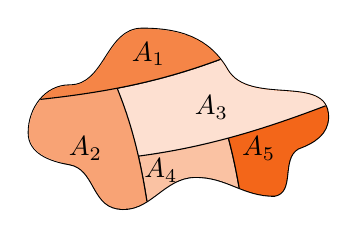
\begin{tikzpicture}[scale=0.4]
\path
  coordinate (aux0) at (0,1.5)
  coordinate (aux1) at (0,3.5)
  coordinate (aux2) at (10,3.5)
  coordinate (aux3) at (9,6)
  coordinate (aux4) at (4,0)
  coordinate (aux5) at (7,0)
  coordinate (aux6) at (2,6)
  coordinate (aux7) at (5,6)
  coordinate (esp1) at (0.2,2.5)
  coordinate (esp2) at (1.5,1.5)
  coordinate (esp3) at (3,0.1)
  coordinate (esp4) at (5.5,1.1)
  coordinate (esp5) at (8,0.5)
  coordinate (esp6) at (8.75,2)
  coordinate (esp7) at (9.7,3)
  coordinate (esp8) at (6.5,4.5)
  coordinate (esp9) at (3.8,5.8)
  coordinate (esp10) at (1.5,4)
  ;
\draw[line width=0.8pt]
  (esp1) to[out=-90,in=170]
  (esp2) to[out=-10,in=170]
  (esp3) to[out=-10,in=180]
  (esp4) to[out=0,in=180]
  (esp5) to[out=10,in=-150]
  (esp6) to[out=20,in=-90]
  (esp7) to[out=90,in=-60]
  (esp8) to[out=120,in=0]
  (esp9) to[out=180,in=0]
  (esp10) to[out=180,in=90]
  cycle;    
\clip
  (esp1) to[out=-90,in=170]
  (esp2) to[out=-10,in=170]
  (esp3) to[out=-10,in=180]
  (esp4) to[out=0,in=180]
  (esp5) to[out=10,in=-150]
  (esp6) to[out=20,in=-90]
  (esp7) to[out=90,in=-60]
  (esp8) to[out=120,in=0]
  (esp9) to[out=180,in=0]
  (esp10) to[out=180,in=90]
  cycle;    
\filldraw[fill=ocre!40]
  (aux4) to[bend right=10]
  (aux6) --
  (aux7) to[bend left=10]
  (aux5) -- cycle;
\filldraw[fill=ocre]
  (aux5) to[bend right=10]
  (aux7) --
  (10,6) --
  (10,0) -- cycle;
\filldraw[fill=ocre!20]
  (aux0) -- 
  (aux1) to[bend right=10]
  (aux3) --
  (10,6) -- 
  (aux2) to[bend left=10] cycle;
\filldraw[fill=ocre!60]
  (0,0) -- 
  (aux4) to[bend right=10]
  (aux6) --
  (0,6) -- 
  (0,0) -- cycle;
\filldraw[fill=ocre!80]
  (0,6) -- 
  (aux1) to[bend right=10]
  (aux3) --
  (0,6) -- cycle;
\node at (4,5) {$A_1$};  
\node at (2,2) {$A_2$};  
\node at (6,3.3) {$A_3$};  
\node at (4.4,1.3) {$A_4$};  
\node at (7.5,2) {$A_5$};  
\node at (7,5) {$\Omega$};  
\end{tikzpicture}
\end{center}
\end{minipage}

\end{definition}


\begin{proposition} Soit $n$ un entier naturel non nul et $A_1$, $A_2$, ..., $A_n$ des ensembles finis deux à deux disjoints.
\[ \Card(A_1 \cup A_2 \cup \ldots  \cup A_n)= \Card(A_1) + \Card(A_2)+\ldots + \Card(A_n)= \sum_{i=1}^n \Card(A_1)\]
\vspace{-0.5cm}\end{proposition}

Une approche possible du dénombrement est d'établir une disjonction de cas pour découper le problème que l'on étudie en d'autres problèmes plus petits que l'on sait dénombrer. Ceci rappelle naturellement la \textbf{formule des probabilités totales}.

\begin{example}Un tournoi de mathématiques est organisé entre 256 joueurs. A chaque manche du tournoi, les participants sont répartis en groupes de 4 candidats et chaque groupe se voit alors attribuer une épreuve à l'issue de laquelle un seul candidat parmi les 4 du groupe pourra se qualifier. A la fin de ce tournoi, il n'y a qu'un seul vainqueur. Combien d'épreuves auront lieu au total ?
\begin{itemize}
\item Notons $E_1$ les épreuves de la première manche. Puisqu'il y a 256 candidats répartis en groupe de 4, il y aura $\frac{256}{4}$ soit 64 épreuves, à l'issue desquelles il restera 64 participants. On a $\Card(E_1)=64$.
\item Notons $E_2$ les épreuves de la deuxième manche. Puisqu'il reste 64 candidats répartis en groupe de 4, il y aura $\frac{64}{4}$ soit 16 épreuves, à l'issue desquelles il restera donc 16 participants. On a $\Card(E_2)=16$.
\item De même, si l'on note $E_3$ et $E_4$ le nombre d'épreuves aux troisièmes et quatrièmes manches, on a $\Card(E_3)=4$ et $\Card(E_4)=1$.
\end{itemize}
Les ensembles $E_1$, $E_2$, $E_3$ et $E_4$ sont disjoints : il n'est pas possible qu'une épreuve se déroule sur deux manches différentes. Par ailleurs, l'union de ces ensembles constitue l'ensemble de toutes les épreuves. Ainsi, le cardinal de l'ensemble de toutes les épreuves de la compétition est égal à la somme des cardinaux de ces 4 ensembles. Il y a donc $64+16+4+1$ soit 85 épreuves dans cette compétition.\end{example}
Tout ce raisonnement peut vous sembler inutilement compliqué pour une situation aussi simpliste que celle-là, mais il faut parfois savoir préciser à outrance les objets et les ensembles que l'on manipule pour être certains que les outils mathématiques que nous utilisons sont les bons.

\begin{proposition}[Formule du crible]
Soit $A$ et $B$ des ensembles finis
\[ \Card(A \cup B) = \Card(A) + \Card(B) - \Card( A\cap B)\]\vspace{-0.5cm}\end{proposition}
\begin{minipage}{0.65\linewidth}
Si l'on compte le nombre d'éléments de $A$ et que l'on ajoute le nombre d'éléments de $B$, certains éléments ont alors été compté deux fois : ceux communs à $A$ et $B$ (c'est-à-dire les éléments de $A\cap B$).

En retirant le nombre d'éléments de cette intersection à notre compte, on obtient alors le nombre d'éléments de l'union.
\end{minipage}\hfill\begin{minipage}{0.3\linewidth}
\newcommand{\A}{(0,0) ++(135:2) circle (2)}
\newcommand{\B}{(0,0) ++(45:2) circle (2)}
\begin{tikzpicture}[scale=0.6]

\draw [thick,black] \A ; 
\draw [thick,black] \B ; 
 \fill[ocre!40, opacity=0.5] \A; \fill[blue!40, opacity=0.5] \B;
 \node at (-2,0) {$A$};
  \node at (2,0) {$B$};
  \node at (0,1) {$A\cap B$};
  
\end{tikzpicture}
\end{minipage}

Encore une fois, la liaison est à faire avec les probabilités et la formule $\mathbb{P}(A\cup B)=\mathbb{P}(A)+\mathbb{P}(B)-\mathbb{P}(A \cap B)$.

\begin{example}Pour accompagner leurs frites à la cantine, 150 élèves choisissent leur sauce entre ketchup et mayonnaise (éventuellement les deux). On suppose que tous les élèves ont pris au moins une sauce. Par ailleurs, 92 élèves ont pris du ketchup et 97 ont pris de la mayonnaise. Combien ont pris les deux sauces ?

Notons $K$ l'ensemble des élèves ayant pris du ketchup et $M$ l'ensemble des élèves ayant pris de la mayonnaise. On a alors $\Card(K)=92$ et $\Card(M)=97$. De plus, chaque élève ayant pris au moins une sauce, on a alors $\Card(K \cup M)=150$. Or, $\Card(K \cup M)=\Card(K)+\Card(M)-\Card(K \cap M)$. \\Ainsi, $\Card(K\cap M)=97+92-150=49$. 49 élèves ont pris à la fois du ketchup et de la mayonnaise.\end{example}
\newpage
\subsection{Produit cartésien}

\begin{definition} Soit $A$ et $B$ deux ensembles.
 
 \begin{itemize}
 \item On appelle \textbf{produit cartésien} de $A$ et $B$, noté $A \times B$ ($A$ "croix" $B$), l'ensemble composé des couples $(a;b)$ avec $a \in A$ et $b \in B$. 
 \item Le produit cartésien $A\times A$ est également noté $A^2$.
\end{itemize}\end{definition}

\begin{example}On considère les ensembles $A=\{2;5;9\};$ et $B=\{3;5\}$.
\begin{itemize}
\item  Les éléments de $A \times B$ sont $(2;3)$, $(2;5)$, $(5;3)$, $(5;5)$, $(9;3)$ et $(9;5)$.
\item Les éléments de $B \times A$ sont $(3:2)$, $(3;5)$, $(3;9)$, $(5;2)$, $(5;5)$, $(5;9)$.
\item Les éléments de $B^2$ sont $(3;3)$, $(3;5)$, $(5;3)$ et $(5;5)$.
\end{itemize}\end{example}

On remarque sur cet exemple que le produit cartésien n'est pas commutatif !

\begin{definition} La notion de \textbf{produit cartésien} s'étend naturellement à plus de deux ensembles. 
\begin{itemize}
 \item Soit $n$ un entier naturel supérieur ou égal à 2. le produit cartésien de $n$ ensembles $A_1$, $A_2$, ..., $A_n$ est l'ensemble des $n$-uplets $(a_1;a_2;\ldots;a_n)$ avec $a_1 \in A_1$, $a_2 \in A_2$, ... $ a_n \in A_n$.
 \item Le produit cartésien $A \times A \times ... \times A$ où $A$ apparaît $n$ fois est noté $A^n$. Ses éléments sont appelés les $n$-\textbf{uplets} de $A$.\end{itemize}
\end{definition}

\begin{example} On considère les ensembles $A=\{1;2;4\}$, $B=\{3;7;14\}$ et $C=\{1;3\}$.
\begin{itemize}
\item $(1;7;3) \in A \times B \times C$ puisque $1 \in A$, $7 \in B$ et $3 \in C$.
\item $(3;7;7;3;14) \in B^5$ puisque $3$, $7$ et 14 sont dans l'ensemble $B$.
\end{itemize}\end{example}

\begin{proposition} Soit $A$ et $B$ des ensembles finis. 
\begin{itemize}
\item $\Card (A \times B)=\Card(A) \times  \Card (B)$.
\item Plus généralement, soit $n$ un entier naturel, $A_1$, $A_2$, ..., $A_n$ des ensembles finis. \[\Card(A_1 \times A_2 \times \ldots \times A_n)=\Card(A_1) \times \Card(A_2) \times \ldots \times \Card(A_n).\]
\item En particulier, pour tout entier naturel $n$, on a $\Card(A^n)=[\Card(A)]^n$.
\end{itemize}\end{proposition}


\begin{example} On reprend les ensembles $A=\{1;2;4\}$, $B=\{3;7;14\}$ et $C=\{1;3\}$. On a
\begin{itemize}
\item $\Card(A \times B)= 3 \times 3 = 9$ ;
\item $\Card(A \times B \times C) = 3 \times 3 \times 2 = 18$ ;
\item $\Card(A^4)=3^4=81$ ;
\item $\Card(C^{10})=2^{10}=1024$.
\end{itemize}\end{example}

\newpage

\begin{proposition} Le produit cartésien est utilisé pour dénombrer des situations où l'ordre des symboles (chiffres, lettres, signes...) est important et où ces symboles peuvent être utilisés plusieurs fois.\end{proposition}

\begin{example} A l'entrée d'un bâtiment est installé un digicode. Pour composer le code, on utilise 4 chiffres compris entre 1 et 6 suivis de deux lettres parmi les lettres A, B, C et D. Un chiffre ou une lettre peuvent être utilisés plusieurs fois. Combien de codes sont possibles ?

On note $A_1=\{1;2;3;4;5;6\}$ et $A_2=\{A;B;C;D\}$. Un digicode est un élément de $A_1^4 \times A_2 ^2$. Le cardinal de cet ensemble est donc $\Card(A_1)^4 \times \Card(A_2)^2 = 6^4 \times 4^2 = 20736$.

Il y a donc 20736 digicodes possibles.\end{example}


\section{Arrangements et permutations}


\begin{definition}Soit $n$ un entier naturel non nul. On note $n!$ (\textbf{factorielle} de $n$) le produit de tous les entiers de 1 à $n$. Ainsi, $n!=n\times (n-1) \times \ldots \times 2 \times 1$.

Par ailleurs, on convient que $0!=1$.\end{definition}

Il est également possible de définir la factorielle par récurrence, en stipulant que $0!=1$ et que, pour tout entier naturel $n$, $(n+1)!=(n+1) \times n!$. Cette version de la factorielle a notamment été rencontrée par les élèves suivants la spécialité NSI lors de leur premier contact avec la récursivité.

\begin{example} $5!=5\times 4 \times 3 \times 2 \times 1 = 120 \quad ;\quad \dfrac{8!}{6!}=\dfrac{8 \times 7 \times 6!}{6!}=8\times 7 = 56$.\end{example}

\begin{definition}Soit $A$ un ensemble fini de cardinal $n$ et $k$ un entier inférieur ou égal à $n$. 

Un $k$-\textbf{arrangement} de $A$ est un $k$-uplet d'éléments distincts de $A$.

Lorsque $k=n$, on parle de \textbf{permutation} de $A$.\end{definition}

\begin{example} On considère l'ensemble $A=\{1;3;4;5;7;10\}$. 
\begin{itemize}
\item $(7;10;3)$ est un 3-arrangement de $A$. 
\item $(10;5;4;1)$ est un 4-arrangement de $A$. 
\item En revanche, $(7;10;1;7)$ n'est pas un arrangement de $A$ car l'élément $7$ y apparaît deux fois. 
\item $(3;7;4;5;1;10)$ est par ailleurs une permutation de $A$ puisque tous les éléments de $A$ y apparaissent.
\end{itemize}\end{example}

 
 \begin{proposition}Soit $A$ un ensemble fini de cardinal $n$ et $k$ un entier inférieur ou égal à $n$. 
 
 Le nombre de $k$-arrangements de $A$ vaut $\dfrac{n!}{(n-k)!}$.
 
 En particulier, le nombre de permutation de $A$ vaut $n!$.\end{proposition}
 
\begin{demonstration} Pour construire un $k$-uplet d'éléments distincts de $A$, on a
 \begin{itemize}
 \item $n$ choix pour le premier élément
 \item $n-1$ choix pour le deuxième
 \item ...
 \item $n-(k-1)$ pour le $k$-ième
 \end{itemize}
 Le nombre de $k$ arrangements de $A$ vaut donc $n \times (n-1) \times \ldots \times n-(k+1)$, ce que l'on peut réécrire en 
 \[ n \times (n-1) \times \ldots \times (n-(k-1)) \times \dfrac{(n-k) \times (n-k-1)\times \ldots \times 2 \times 1}{(n-k) \times (n-k-1)\times \ldots \times 2 \times 1}=n \times (n-1) \times \ldots \times (n-(k-1)) \times \dfrac{(n-k)!}{(n-k)!}\]
 d'où
 \[n \times (n-1) \times \ldots \times( n-(k-1)) \times \dfrac{(n-k) \times (n-k-1)\times \ldots \times 2 \times 1}{(n-k) \times (n-k-1)\times \ldots \times 2 \times 1}=\dfrac{n!}{(n-k)!}.\]\end{demonstration}
 
\begin{example} On considère l'ensemble $A=\{1;3;4;5;7;9;11\}$, de cardinal 7. 

Le nombre de $3$-arrangements de $A$ vaut $7 \times 6 \times 5 = 210$.\end{example}


 
\begin{proposition} Les arrangements sont utilisés pour dénombrer des situations où l'ordre des objets (chiffres, nombres, lettres, signes,...) est important mais où chaque objet ne peut être utilisé qu'une seule fois.\end{proposition}

\begin{example}Une cours hippique réunit 8 jockeys et leurs chevaux. Le "quarté dans l'ordre" est un pari qui consiste à deviner les quatre premiers chevaux arrivés dans l'ordre. Combien de paris différents est-il possible de réaliser ?
 \begin{itemize}
 \item On a 8 choix pour le premier cheval arrivé.
 \item Il reste 7 choix pour le deuxième, 6 pour le troisième et 5 pour le quatrième.
 \item Le nombre total de paris est donc $8 \times 7 \times 6 \times 5 = 1680$.
 \end{itemize}
 Formellement, si on nomme $A$ l'ensemble des chevaux de la course, un quarté dans l'ordre est un 4-arrangement de $A$.\end{example}
 

 \section{Combinaisons d'un ensemble fini}
 
 \begin{definition} Une \textbf{partie} ou \textbf{combinaison} d'un ensemble fini $A$ est un ensemble inclus dans $A$. L'ensemble des parties de $A$ est noté $\mathcal{P}(A)$.\end{definition}


\begin{example} Soit $A=\{1;2;3\}$. Les parties de $A$ sont $\varnothing$, $\{1\}$, $\{2\}$, $\{3\}$, $\{1;2\}$, $\{1;3\}$, $\{2;3\}$ et $\{1;2;3\}$. Elles sont au nombre de $8$

Attention à ne pas oublier l'ensemble vide $\varnothing$ et l'ensemble complet $A$ lui-même en établissant cette liste.\end{example} 
 
 \begin{proposition}
Soit $A$ un ensemble fini de cardinal $n$. Le nombre de parties de $A$ est $2^n$.\end{proposition}
 
\begin{demonstration} Nous allons montrer qu'il y a autant de parties de $A$ que de $n$-uplets de l'ensemble $\{0;1\}^n$. Puisque $\{0;1\}$ possède 2 éléments, le cardinal de $\{0;1\}^n$ vaut donc $2^n$.
 
 Pour cela, à chaque partie de $A$, on fait correspondre un élément de $\{0;1\}^n$ de telle sorte que deux parties différentes de $A$  sont associés à deux $n$-uplets différents de $\{0;1\}$. On dit qu'on réalise une bijection entre $\mathcal{P}(A)$ et $\{0;1\}^n$.
 
 L'idée : Pour chaque élément de $A$, on a deux choix pour construire une partie de $A$ : soit cet élément appartient à la partie que l'on construit, soit il ne lui appartient pas. 

\newpage 
 
 On a donc
 \begin{itemize}
 \item 2 choix pour le premier élément de $A$
 \item 2 choix pour le deuxième élément...
 \item ...
 \item 2 choix pour le $n$-ième élément de $A$.
 \end{itemize}
 Ainsi, le cardinal de $\mathcal{P}(A)$ vaut $2\times 2 \times \ldots \times 2 = 2^n$.
 
 
De manière formelle : Notons $a_1$, $a_2$ , ..., $a_n$ les éléments de $A$. 
  Soit $B$ une partie de $A$. On construit un $n$-uplet $(b_0;b_1;...;b_n)$ de $\{0;1\}$ comme suit : pour tout entier naturel $i$ entre 1 et $n$
  \begin{itemize}
  \item $b_i=1$ si $a_i \in B$
  \item $b_1=0$ sinon.
  \end{itemize}
Chaque partie de $A$ est ainsi associé de manière unique à un $n$-uplet de $\{0;1\}$ et réciproquement. Les cardinaux de $\mathcal{P}(A)$ et $\{0;1\}^n$ sont donc égaux.\end{demonstration}



\begin{definition} Soit $A$ un ensemble fini à $n$ éléments et $k$ un entier naturel $n$. 

Le nombre de combinaisons à $k$ éléments de $A$ est noté $\dbinom{n}{k}$ et se lit "$k$ parmi $n$". 

Les nombres $\dbinom{n}{k}$ sont appelés coefficients binomiaux\end{definition}

\begin{example}Soit $A=\{1:2:3:4:5\}$. Les parties à deux éléments de $A$ sont $\{1;2\}$, $\{1;3\}$, $\{1;4\}$, $\{1;5\}$, $\{2;3\}$, $\{2;4\}$, $\{2;5\}$, $\{3;4\}$, $\{3;5\}$ et $\{4;5\}$. Il y en a 10 : ainsi, $\dbinom{5}{2}=10$.\end{example}

Attention, l'ordre n'a pas d'importance lorsque l'on parle de partie d'un ensemble : le sous-ensemble $\{1;2\}$ est le même que le sous-ensemble $\{2;1\}$.


\begin{proposition} Soit $n$ et $k$ deux entiers naturels.
\begin{itemize}
\item Si $k > n$, $\dbinom{n}{k}=0$ ;
\item Sinon, $\dbinom{n}{k} = \dfrac{n!}{k!(n-k)!}$.
\end{itemize}
.\end{proposition}

\begin{demonstration}On sait qu'il y a $\dfrac{n!}{(n-k)!}$ $k$-arrangements de $A$. Cependant, plusieurs $k$-arrangements utilisent les mêmes éléments de $A$ (par exemple, les couples (1;2) et (2;1) utilisent les nombres 1 et 2). Etant donné une partie de $A$ à $k$ éléments, on peut construire $k!$ arrangements différents : on a $k$ choix pour le premier élément, $k-1$ pour le deuxième, etc.

Ainsi, le nombre de $k$-arrangements est $k!$ fois plus grand que la nombre de combinaisons à $k$ éléments. Ainsi, le nombre de combinaisons à $k$ élements est égale au nombre de $k$-arrangements divisé par $k!$, soit $\dfrac{n!}{k!(n-k)!}$.\end{demonstration}

\newpage

\begin{example} Soit $A=\{1;2;3;4\}$. 

Le nombre de parties de $A$ à deux éléments vaut $\dbinom{4}{2}=\dfrac{4!}{2!(4-2)!}=\dfrac{4!}{2!2!}=\dfrac{24}{2 \times 2}=6$.\\ Ces parties sont $\{1;2\}$, $\{1;3\}$, $\{1;4\}$, $\{2;3\}$, $\{2;4\}$ et $\{3;4\}$.\end{example}



\begin{proposition} Soit $n$ un entier naturel non nul. 

\begin{tabularx}{\linewidth}{X|X}
Pour tout entier naturel $k \leqslant n$, $\dbinom{n}{k}=\dbinom{n}{n-k}$. & $\dbinom{n}{0}=\dbinom{n}{n}=1$. \\
\hline
Si $n\geqslant 1$, $\dbinom{n}{1}=\dbinom{n}{n-1}=n$. & Si $n\geqslant 2$, $\dbinom{n}{2}=\dbinom{n}{n-2}=\dfrac{n(n-1)}{2}$.
\end{tabularx}

\end{proposition}

\begin{demonstration} (Avec la formule) :
\begin{itemize}
\item Pour tout entier naturel $k\leqslant n$, $\dbinom{n}{n-k}=\dfrac{n!}{(n-k)!(n-(n-k))!}=\dfrac{n!}{k!(n-k)!}=\dbinom{n}{k}$.
\item D'après le premier point, on a bien $\dbinom{n}{0}=\dbinom{n}{n-0}=\dbinom{n}{n}$. Or, $\dbinom{n}{0}=\dfrac{n!}{0!n!}=\dfrac{n!}{n!}=1$.
\item D'après le premier point,  $\dbinom{n}{1}=\dbinom{n}{n-1}$. Or, $\dbinom{n}{1}=\dfrac{n!}{1!(n-1)!}=\dfrac{n!}{(n-1)!}=\dfrac{n \times (n-1)!}{(n-1)!}=n$.
\item D'après le premier point,  $\dbinom{n}{2}=\dbinom{n}{n-2}$.

 Or, $\dbinom{n}{2}=\dfrac{n!}{2!(n-2)!}=\dfrac{n!}{2(n-2)!}=\dfrac{n(n-1) \times (n-2)!}{2(n-1)!}=\dfrac{n(n-1)}{2}$.
\end{itemize}\end{demonstration}






\begin{demonstration} (Démonstration combinatoire)

\begin{itemize}
\item Choisir $k$ objets parmi $n$ revient à exclure $n-k$ objets parmi ces $n$ objets. Ainsi, $\dbinom{n}{k}=\dbinom{n}{n-k}$.
\item Il n'existe qu'un seul ensemble à 0 élément, il s'agit de l'ensemble vide $\varnothing$. De la même manière, si $A$ est un ensemble à $n$ éléments, la seule partie de $A$ ayant $n$ éléments est l'ensemble $A$ lui-même.\\  Ainsi, $\dbinom{n}{0}=\dbinom{n}{n}=1$.
\item Si $A$ est un ensemble fini $\{a_1;a_2;\ldots ;a_n\}$ de cardinal supérieur ou égal à 1, les parties à 1 élément de $A$ sont simplement les singletons $\{ a_1\}$, $\{a_2\}$, ... , $\{a_n\}$. 

Ainsi, $\dbinom{n}{1}=\dbinom{n}{n-1}=n$.
\item Soit $A$ un ensemble de cardinal $n\geqslant 2$. Pour construire une partie à 2 éléments de $A$, on choisit un premier élément ($n$ choix possibles) puis un second ($n-1$ choix). En faisant ainsi, on peut construire $n(n-1)$ couples d'éléments de $A$. Or, l'ordre n'ayant pas d'importance, il est possible d'inverser l'ordre dans lequel on choisit les éléments de $A$. \\ Le nombre de combinaisons de $A$ à 2 éléments vaut donc $\dfrac{n(n-1)}{2}$
\end{itemize}\end{demonstration}

\begin{example} $\dbinom{100}{98}=\dbinom{100}{2}=\dfrac{100 \times 99}{2}= 4950$.\end{example}



\begin{proposition}Les combinaisons sont utilisées pour dénombrer les situations où l'ordre des objets n'est pas important - lorsque l'on tire simultanément plusieurs personnes ou objets au hasard par exemple - et qu'un objet ne peut être utilisé qu'une seule fois.\end{proposition}

\begin{example} A la belote, on utilise un jeu de 32 cartes. Chaque carte est déterminé par sa couleur (Pique, Trèfle, Carreau, Coeur) et sa valeur (As, Roi, Dame, Valet, 10, 9, 8, 7). Pour le premier tour de distribution, chaque joueur reçoit 5 cartes, que l'on appelle une main. Combien existe-t-il de mains comportant exactement 2 as ?

L'ordre de distribution des cartes n'a pas d'importance ici : recevoir un as en première carte ou en deuxième carte n'a pas d'influence, on utilise donc les combinaisons.
\begin{itemize}
\item La main est composée de 2 as, choisis parmi 4, ce qui donne $\dbinom{4}{2}=\dfrac{4!}{2!(4-2)!}=\dfrac{4!}{2!2!}=\dfrac{24}{4}=6$ possibilités.
\item Il reste 3 cartes à déterminer, choisis parmi les 28 cartes qui ne sont pas des as. \\
Cela donne $\dbinom{28}{3}=\dfrac{28!}{3!(28-3)!}=\dfrac{28!}{3!25!}=\dfrac{28\times 27 \times 26}{3 \times 2 \times 1}=3276$.
\item Au total, cela fait $6\times 3276 =19656$ mains de 5 cartes contenant exactement 2 as.
\end{itemize}\end{example}



\begin{proposition}Soit $n$ un entier naturel supérieur ou égal à 2 et $k$ un entier tel que $1\leqslant k\leqslant n-1$. On a alors
\[ \dbinom{n-1}{k-1}+\dbinom{n-1}{k} = \dbinom{n}{k}.\]
Cette relation s'appelle la relation de Pascal.\end{proposition}

\begin{demonstration}[Avec la formule] : On a
\[ \dbinom{n-1}{k-1}+\dbinom{n-1}{k}=\dfrac{(n-1)!}{(k-1)!(n-1-(k-1))!}+\dfrac{(n-1)!}{k!(n-1-k)!}\]

On multiplie le premier quotient par $\dfrac{k}{k}$ et le second par $\dfrac{n-k}{n-k}$, ce qui donne
\[\dbinom{n-1}{k-1}+\dbinom{n-1}{k}=\dfrac{k \times (n-1)!}{k\times (k-1)! \times (n-1)!}+\dfrac{(n-k) \times (n-1)!}{k! \times (n-k-1)! \times (n-k)}\]
Or, $k\times (k-1)!=k!$, $(n-k-1) \times (n-k)=(n-k)!$. Ainsi,

\[\dbinom{n-1}{k-1}+\dbinom{n-1}{k} = \dfrac{k \times (n-1)!}{k!(n-k)!}+\dfrac{(n-k) \times (n-1)!}{k!(n-k)!}=\dfrac{n \times (n-1)!}{k! (n-k)!}=\dfrac{n!}{k!(n-k)!}=\dbinom{n}{k}\]\end{demonstration}

\begin{demonstration}[Combinatoire] : Soit $A$ un ensemble fini à $n$ éléments et $a\in A$. Soit $k$ un entier naturel compris entre 1 et $n-1$. 

L'ensemble des combinaisons à $k$ éléments, noté $\mathcal{P}_k(A)$, est, par définition, de cardinal $\dbinom{n}{k}$. Il peut se décomposer en deux ensembles disjoints :
\begin{itemize}
\item $P_1$, l'ensemble des combinaisons à $k$ éléments de $A$ qui contiennent l'élément $a$. Il reste donc à choisir $k-1$ éléments parmi les $n-1$ restants. Le cardinal de cet ensemble est donc $\dbinom{n-1}{k-1}$ ;
\item $P_2$, L'ensemble des combinaisons à $k$ éléments de $A$ qui ne contiennent pas l'élément $a$. Il faut donc choisir $k$ éléments parmi les $n-1$ autres éléments. Le cardinal de $P_2$ est donc $\dbinom{n-1}{k}$.
\end{itemize}
On a alors $\mathcal{P}_k(A)=P_1 \cup P_2$ ce qui implique que $\dbinom{n}{k} = \Card(\mathcal{P}_k(A))=\Card(P_1 \cup P_2)$. Or, les ensembles $P_1$ et $P_2$ sont disjoints. Ainsi, $\Card(P_1 \cup P_2)= \Card(P_1)+\Card(P_2)$. 

Autrement dit, on a $\dbinom{n}{k}=\dbinom{n-1}{k-1}+\dbinom{n-1}{k}$.\end{demonstration}


\begin{proposition}La relation de Pascal permet de construire récursivement les coefficients binomiaux. Ces coefficients peuvent être arrangés en triangle et forment ce que l'on appelle le triangle de Pascal.
\vskip5pt
\begin{minipage}{0.45\linewidth}
\begin{center}
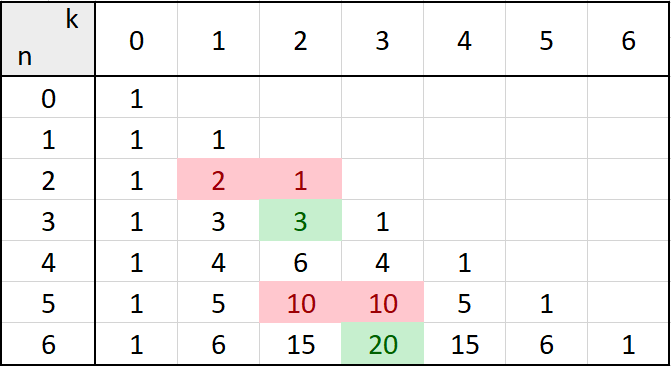
\includegraphics[scale=1.2]{pascal}
\end{center}
\end{minipage}\hfill\begin{minipage}{0.5\linewidth}
Dans ce triangle, on démarre avec un 1 en haut à gauche. Pour compléter chaque cellule, on ajoute alors le nombre au-dessus avec le nombre en haut à gauche. Les cases vides se voient assigner la valeur 0. On peut alors lire les coefficients binomiaux $\dbinom{n}{k}$ dans ce triangle.
\end{minipage}




\end{proposition}

\chapter{Exercices}

\section*{Cardinal d'ensembles}

\begin{exercise}On considère l'ensemble $A=\{5;9;13\}$. Déterminer l'ensemble $B$, disjoint de $A$, tel que $A\cup B =\{1;2;5;8;9;13;14\}$.\end{exercise}

\begin{solution} On prend les éléments de $A \cup B$ qui ne sont pas dans $A$. $B=\{1;2;8;14\}$.\end{solution}


\begin{exercise}On considère deux ensembles $A$ et $B$.
\begin{itemize}
\item Si $\Card(A)=18$, $\Card(B)=23$, $A$ et $B$ étant disjoints, que vaut $\Card(A \cup B)$ ?
\item Si $\Card(A)=12$, $\Card(B)=47$ et $\Card(A \cup B) = 58$, $A$ et $B$ sont-ils disjoints ?
\item Si $\Card(A)=14$ et $\Card(A \cup B) = 27$, quel est le nombre minimal d'éléments dans $B$ ?
\end{itemize}\end{exercise}

\begin{solution}\hspace{0pt}
\begin{itemize}
\item Puisque $A$ et $B$ sont disjoints, $\Card(A \cup B)=\Card(A) + \Card(B) = 18 + 23 = 41$.
\item On a $\Card(A)+\Card(B)=47+12=59 \neq \Card(A \cup B)$, $A$ et $B$ ne sont pas disjoints.
\item $B$ comporte au moins $27-24=13$ éléments.\end{itemize}
\end{solution}



\begin{exercise}À leur entrée en L1, les étudiants choisissent une langue (anglais ou allemand) et une option (informatique, chimie ou astronomie). Dans un groupe d'étudiants, 12 étudiants sont inscrits en astronomie, 15 en chimie, 16 étudient l'allemand. Par ailleurs, 8 inscrits en astronomie et 3 inscrits en informatique étudient l'anglais, 6 inscrits en chimie étudient l'allemand.

Indiquer la répartition des étudiants par discipline, ainsi que le nombre total d'étudiants dans le groupe.\end{exercise}



\begin{solution}Il est possible de résoudre cet exercice en utilisant un tableau.

\begin{center}
\begin{tabular}{|c|c|c|c|c|}
\hline
 & Informatique & Chimie & Astronomie & Total \\
 \hline
 Anglais &3&9&8&20 \\
 \hline
 Allemand &6&6&4&16\\
 \hline
 Total &9&15&12&36 \\
 \hline \end{tabular}
\end{center}\end{solution}




\begin{exercise}Pour tout entier naturel $n$, on note $A_n$ l'ensemble des solutions de l'équation $x^2-n=0$. 

Déterminer $\Card(A_0 \cup A_1 \cup A_2 \cup \ldots \cup A_n)$.	
\end{exercise}

\begin{solution}Pour tout entier naturel $n$, on note $A_n$ l'ensemble des solutions de l'équation $x^2-n=0$. Ainsi, $A_0=\{0\}$ et pour tout entier naturel non nul, $A_n=\{-\sqrt{n} ; \sqrt{n}\}$. Ces ensembles sont disjoints et de cardinal 2.

Ainsi, $\Card(A_0 \cup A_1  \cup \ldots \cup A_n)=\Card(A_0)+\Card(A_1)+\ldots + \Card(A_n)=1+2+2+\ldots + 2=2n+1$.\end{solution}





\begin{exercise}Soit $A=\{5;7\}$ et $B=\{7;9;10\}$. Donner l'ensemble des éléments de $A\times B$, de $B \times A$, de $A^3$ et de $B^2$.\end{exercise}

\begin{solution} On a
\begin{itemize}
\item $A\times B=\{(5;7), (5;9), (5;10), (7;7), (7;9), (7;10)\}$, 
\item $B \times A = \{(7;5),(7;7), (9;5), (9;7), (10;5), (10;7)\}$, 
\item $A^3 = \{(5;5;5),(5;5;7),(5;7;5), (5;7;7), (7;5;5),(7;5;7),(7;7;5),(7;7;7)\}$,
\item $B^2=\{(7;7),(7;9),(7;10),(9;7),(9;9),(9;10),(10;7),(10;9),(10;10)\}$.
\end{itemize}\end{solution}



\begin{exercise}
Soit $A$ et $B$ deux ensembles finis tels que $\Card(A \times B)=299$ et 
$\Card(A \cup B)=37$. Les ensembles $A$ et $B$ sont-ils disjoints ?\end{exercise}

\begin{solution}$299 = 1 \times 299 = 13 \times 23$. Les seules possibilités pour les cardinaux de $A$ et $B$ sont donc 1, 13, 23 et 299.

 Or, $13+23=39$ et $1+299=300$, qui sont différents de 37. Ainsi, $A$ et $B$ ne sont pas disjoints.
\end{solution}



\begin{exercise}Parmi tous les nombres de 1 à 1000, combien s'écrivent avec le chiffre 9 ?\end{exercise}

\begin{solution}Comptons le nombre de nombres n'ayant aucun 9 dans leur écriture. Il y a 9 choix pour le premier chiffre, 9 pour le deuxième, 9 pour le troisième soit $9^3=729$ possibilités. Ainsi, les nombres qui s'écrivent avec un 9 sont au nombre de $1000-729=271$.\newpage \end{solution}




\begin{exercise}En informatique, un octet est une succession de 8 bits, chaque bit ne pouvant prendre que deux valeurs, 0 ou 1. Un octet est donc un 8-uplet de  $\{0;1\}$.
\begin{enumerate}
\item Combien d'octets différents existe-t-il ?
\item Dans le système RGB, une couleur est codée à l'aide de 3 octets désignant respectivement les niveaux de rouge, de vert et de bleu. Combien de couleurs différentes est-il ainsi possible de coder ?
\item Une adresse IPv4 est codée sur 4 octets. On considère un sous-réseau dont le masque est 255.255.0.0, c'est-à-dire que toutes les adresses IP des ordinateurs de ce sous-réseau commencent par les deux mêmes octets. Par ailleurs, les adresses se terminant par les octets 0.0 et 255.255 sont réservées respectivement au réseau et au broadcast. Combien de machines différentes peut-on brancher sur un tel réseau ?
\end{enumerate}\end{exercise}

\begin{solution}Il existe $2^8$ soit 256 octets. Il est alors possible de coder $256^3$ soit 16777216 couleurs dans le système RGB.

Pour établir une adresse IPv4 de ce sous-réseau, on a 256 possibilités pour le troisième octet et 256 pour le quatrième. Il faut alors retirer les deux adresses réservées. Il est alors possible de connecter $256^2-2$ soit $65534$ machines au réseau.\end{solution}




\begin{exercise}Dans un restaurant figurent au menu
\begin{itemize}
\item 12 entrées : 3 avec viande, 3 avec poisson et 6 végétariennes ;
\item 20 plats : 10 avec viande, 6 avec poisson et 4 végétariens.
\end{itemize}
Un client commande au hasard de manière uniforme et indépendante une entrée et un plat.
\begin{enumerate}
\item Quelle est la probabilité que le menu de ce client soit végétarien ?
\item Quelle est la probabilité que son menu soit composé d'une entrée et d'un plat tous deux sans poisson ?
\item Quelle est la probabilité que l'entrée et le plat soit de nature différente (par exemple une entrée avec viande et un plat végétarien) ?
\end{enumerate}\end{exercise}

\begin{solution}Il y a $12 \times 20$ soit $240$ menus au total. Il y a par ailleurs $6 \times 4$ menus végétariens. \\La probabilité que le menu soit végétarien est de $\dfrac{24}{240}$ soit $\dfrac{1}{10}$.

Il y a 9 entrées sans poissons et 14 plats sans poissons, soit $9\times 14$ menus sans poisson. \\La probabilité que le menu soit sans poisson est de $\dfrac{9\times 14}{240}=\dfrac{21}{40}$.

Le nombres de menus ayant entrée et plat différents est $3 \times 10+3 \times 14 +6 \times 16$ soit 168. \\La probabilité de l'événement recherché est donc $\dfrac{168}{240}$ soit $\dfrac{7}{10}$.\end{solution}





\begin{exercise}Un trigramme est une figure composée de trois lignes parallèles, chacune pouvant être coupée en deux morceaux ou non. Le drapeau de la Corée du Sud présente par exemple quatre trigrammes entourant un Taiju bleu et rouge.
\begin{enumerate}
\item Combien de trigrammes différents peut-on constituer ?

\item Construire les trigrammes ne figurant pas sur le drapeau.

\begin{center}

\includegraphics[scale=0.25]{coree}
\end{center}
\end{enumerate}
\end{exercise}

\begin{solution}Il est possible de constituer 8 trigrammes. \end{solution}



\section*{Arrangements et permutations}

\begin{exercise}On considère l'ensemble $A=\{1;3;7;11\}$. Donner tous les 2-arrangements de $A$. Combien y en a-t-il ?\end{exercise}

\begin{solution}Les 2-arrangements de $A$ sont (1;3), (1;7), (1;11), (3;1), (3;7); (3;11), (7;1), (7;3), (7;11), (11;1), (11;3), (11;7). Il y en a 12.\end{solution}



\begin{exercise}On considère l'ensemble $A=\{c;o;s\}$ Donner toutes les permutations de $A$. Combien y en a-t-il ?\end{exercise}

\begin{solution}Les permutations de $A$ sont (s;i;n), (s;n;i), (i;s;n), (i;n;s), (i;s;n), (i;n;s). Il y en a 6.\end{solution}




\begin{exercise}
On considère l'ensemble $A=\{1;3;7;9;11\}$.
\begin{enumerate}
\item Donner deux éléments de $A^3$. Combien en existe-t-il ?
\item Donner deux 3-arrangements d'éléments de $A$. Combien en existe-t-il ?
\item Donner deux permutations de $A$. Combien en existe-t-il ?
\end{enumerate}\end{exercise}

\begin{solution}\hspace{0pt}
\vspace{-0.5cm}
\begin{itemize}
\item $(1;3;3)$ et $(7;7;1)$ sont deux éléments de $A^3$. Il en existe $5^3$ soit 125.
\item $(1;7;11)$ et $(7;9;1)$ sont deux 3-arrangements d'éléments de $A$. Il en existe $5 \times 4 \times 3 = 60$.
\item $(1;7;3;11;9)$ et $(11;9;3;7;1)$ sont deux permutations de $A$. Il en existe $5!=120$.
\end{itemize}\end{solution}



\begin{exercise}Une course de 8 athlètes a lieu. 
\begin{enumerate}
\item Combien y a-t-il de podiums possibles ? 
\item Combien y a-t-il de classements complets possibles ?
\item Anne a participé à la course et a terminé sur le podium. Sachant cette information, combien de classements complets sont possibles ?
\end{enumerate}\newpage \end{exercise}

\begin{solution}Il y a $8 \times 7 \times 6$ soit 336 podiums possibles. Il y a $8!$ soit 40320 classements possibles.

Classons les 7 autres personnes : il y a 7! classement possibles. Il faut alors insérer Anne en première, deuxième ou troisième position. Le nombre de classements complets vaut alors $3 \times 7!$ soit 15120.\end{solution}




\begin{exercise}Le professeur souhaite envoyer ses élèves au tableau pour corriger des exercices. Il y a 3 exercices à corriger et 30 élèves dans la classe.
\begin{enumerate}
\item Combien y a-t-il de configurations possibles si un même élève ne peut pas venir deux fois au tableau ?
\item Même question si un élève peut être interrogé sur plusieurs exercices.
\end{enumerate}\end{exercise}


\begin{solution}Si un élève ne peut pas venir deux fois au tableau, il y a 30 possibilités pour le premier élèves, 29 pour le deuxième et 28 pour le troisième, soit un total de $30 \times 29 \times 28=24360$ configurations.

Si, en revanche, un élève peut passer plusieurs fois, il y a 30 choix pour chaque exercice, soit un total de $30^3=27000$ configurations.\newpage \end{solution}



\begin{exercise}Deux groupes d'étudiants se rendent au cinéma. Le premier est composé de 6 personnes et le deuxième de 4 personnes. Les étudiants s'installent sur une rangée de dix places.
\begin{enumerate}
\item Combien de configurations différentes existe-t-il ?
\item Les deux groupes ne veulent pas être séparés. Combien de configurations sont possibles ?
\end{enumerate}\end{exercise}

\begin{solution}Il existe $10!=3628800$ configurations possibles.

Si les étudiants ne souhaitent pas se séparer, il y a deux situations possibles.
\begin{itemize}
\item On place le premier groupe puis le deuxième. Il y a $6!$ manières de placer le premier groupe et $4!$ pour le deuxième.
\item On place le deuxième groupe puis le premier, on obtient le même nombre de placements.
\item Le nombre de configurations possibles est donc de $2 \times 6! \times 4! = 34560$.
\end{itemize}\end{solution}




\begin{exercise}
On dispose des lettres de SAINTEX. On souhaite construire de nouveaux mots à l'aide de ces lettres, sans s'intéresser au sens de ces mots. On peut par exemple former les mots EXTIA ou SINETAX.
\begin{enumerate}
\item Combien de mots de 4 lettres peut-on former si toutes les lettres peuvent être utilisées autant de fois que l'on veut ?
\item Combien de mots de 4 lettres peut-on former si chaque lettre ne peut être utilisée qu'une seule fois ?
\item Combien de mots de 6 lettres ne commençant pas par la lettre X peut-on former, chaque lettre pouvant être utilisée autant de fois que l'on veut ?
\item Combien de mots de 4 lettres comportant la lettre I existe-t-il, chaque lettre ne pouvant être utilisée qu'une seule fois ?
\end{enumerate}\end{exercise}

\begin{solution}\hspace{0pt}
\vspace{-0.5cm}
\begin{enumerate}
\item On peut former $7^4=2401$ mots.
\item On peut former $7 \times 6 \times 5 \times 4 = 840$ mots.
\item Il y a 6 choix pour la première lettre, puis 7 pour la deuxième, 7 pour la troisième et ainsi de suite. Le nombre de mots est de $6 \times 7^5 = 100842$.
\item On divise les mots selon la position de la lettre I.
\begin{itemize}
\item Si elle est en première position, on a alors 6 choix pour la deuxième lettre, 5 pour la troisième, 4 pour la quatrième, soit 120 possibilités.
\item Le même raisonnement vaut si le O est en position 2, 3 ou 4.
\item Il y a donc 480 possibilités au total.
\end{itemize}
\end{enumerate}\end{solution}



\begin{exercise}[subtitle={(Amérique du Sud 2009)}]

On considère un questionnaire comportant cinq questions. Pour chacune des cinq questions posées, trois propositions de réponses sont faites (A, B et C), une seule d'entre elles étant exacte.

Un candidat répond à toutes les questions posées en écrivant un mot réponse
de cinq lettres.
Par exemple, le mot BBAAC signifie que le candidat a répondu B aux première et deuxième questions, A aux troisième et quatrième questions et C à la
cinquième question.
\begin{enumerate}
\item Combien y-a-t'il de mots-réponses possible à ce questionnaire ?
\item On suppose que le candidat répond au hasard à chacune des cinq questions de ce questionnaire. Calculer la probabilité des évènements suivants :
\begin{itemize}
\item E : " le candidat a exactement une réponse exacte ".
\item F : " le candidat n'a aucune réponse exacte ".
\item G : " le mot-réponse du candidat est un palindrome " (On précise qu'un
palindrome est un mot pouvant se lire indifféremment de gauche à droite
ou de droite à gauche : par exemple, BACAB est un palindrome).\end{itemize}
\end{enumerate}\end{exercise}


\begin{solution}\hspace{0pt}
\vspace{-0.5cm}
\begin{enumerate}
\item Il y a à chaque fois 3 choix par question, soit $3^5$ mots-réponses possibles.
\item 
\begin{itemize}
\item  On distingue selon la position de la bonne réponse.
\begin{itemize}
\item S'il s'agit de la première réponse, il y a $1 \times 2 \times 2 \times 2 \times 2 = 16$ mots-réponses possibles.
\item Le même raisonnement tient s'il s'agit de la deuxième, troisième, quatrième ou cinquième réponse.
\item Au total 80 mots-réponses contiennent exactement une bonne réponse.
\end{itemize}
La probabilité d'avoir exactement une bonne réponse est donc de $\dfrac{80}{243}$.
\item Il y a deux mauvaises réponses par question. La probabilité de n'avoir aucune réponse exacte est donc $\dfrac{2^5}{243}=\dfrac{32}{243}$.
\item Il y a 3 choix pour la première lettre, 3 pour la deuxième et 3 pour la troisième. Il n'y a qu'un choix pour la quatrième qui doit être la même que la deuxième et un seul choix également pour la cinquième qui doit être la même que la première. \\La probabilité d'avoir un palindrome est donc de $\dfrac{3^3}{3^5}=\dfrac{1}{3^2}=\dfrac{1}{9}$.\end{itemize}
\end{enumerate}\end{solution}

\begin{exercise}[subtitle={(Centres étrangers 2024)}]

Un sac opaque contient huit jetons numérotés de 1 à 8, indiscernables au toucher.

À trois reprises, un joueur pioche un jeton dans ce sac, note son numéro, puis le remet dans le sac. Dans ce contexte, on appelle « tirage » la liste ordonnée des trois numéros obtenus.
Par exemple, si le joueur pioche le jeton numéro 4, puis le jeton numéro 5, puis le jeton numéro 1, alors le tirage correspondant est (4; 5; 1).
\begin{enumerate}
\item Déterminer le nombre de tirages possibles.
\item\begin{enumerate}
\item Déterminer le nombre de tirages sans répétition de numéro.
\item En déduire le nombre de tirages contenant au moins une répétition de numéro.\end{enumerate}\end{enumerate}

\end{exercise}

\begin{solution}
L'ordre des tirages est pris en compte et il y a remise entre chaque tirage. Nous avons 8 possibilités pour le premier tirage, 8 pour le deuxième et 8 pour le troisième. Il y a donc $8^3=512$ tirages. possibles.

Le nombre de tirages sans répétition est de $8 \times 7 \times 6 =336$. Le nombre de tirage contenant au moins une répétition est donc de $512-336=176$.\newpage\end{solution}




\section*{Combinaisons d'un ensemble fini}

\begin{exercise}Soit $A=\{1;2;3;4\}$. donner toutes les parties de $A$ à 2 éléments et en déduire la valeur de $\dbinom{4}{2}$.\end{exercise}

\begin{solution}Les parties de $A$ à deux éléments sont $\{1;2\}$, $\{1;3\}$, $\{1;4\}$, $\{2;3\}$, $\{2;4\}$ et $\{3;4\}$.\end{solution}



\begin{exercise}Donner les valeurs de $\dbinom{6}{3}$, $\dbinom{10}{7}$, $\dbinom{14}{11}$,  $\dbinom{9}{4}$, $\dbinom{9}{5}$ et $\dbinom{8}{3}$.\end{exercise}

\begin{solution}\hspace{0pt}
 \begin{itemize}
 \item $\dbinom{6}{3}=\dfrac{6!}{3!3!}=\dfrac{6 \times 5 \times 4 \times 3!}{(3 \times 2 \times 1)3!}=5 \times 4 =20$.

\item $\dbinom{10}{7}=\dfrac{10!}{7!3!}=\dfrac{10 \times 9 \times 8 \times 7!}{(3 \times 2 \times 1)7!}=\dfrac{10 \times 9 \times 8}{3 \times 2} = 5 \times 3 \times 8 = 120$.

\item $\dbinom{14}{11}=\dfrac{14!}{11!3!}=\dfrac{14 \times 13 \times 12 \times 11!}{11! \times (3 \times 2 \times 1)}=14 \times 13 \times 2 = 364$.

\item $\dbinom{9}{4}=\dfrac{9!}{4!5!}=\dfrac{9 \times 8 \times 7 \times 6 \times 5!}{5!(4 \times 3 \times 2 \times 1)}=3 \times 7 \times 6 = 126$.

\item $\dbinom{9}{5}=\dfrac{9!}{5!4!}=126$ d'après le calcul précédent.

\item $\dbinom{8}{3}=\dfrac{8!}{3!5!}=\dfrac{8 \times 7 \times 6 \times 5!}{5!(1 \times 2 \times 3)}=8\times 7 = 56$.\end{itemize}
\end{solution}




\begin{exercise}Calculer les coefficients binomiaux : $\dbinom{31}{2}$, $\dbinom{279}{279}$, $\dbinom{1457}{0}$, $\dbinom{4321}{4320}$, $\dbinom{101}{99}$.\end{exercise}


\begin{solution}$\dbinom{31}{2}=\dfrac{31 \times 30 }{2} = 465$, $\dbinom{279}{279}=1$, $\dbinom{1457}{0}=1$, $\dbinom{4321}{4320}=4321$, $\dbinom{101}{99}=\dfrac{101 \times 100}{2}=5050$.\end{solution}




\begin{exercise}Pour tout entier naturel $n$, on pose $u_n=\dbinom{2n}{n}$. Montrer que la suite $(u_n)$ est strictement croissante.\end{exercise}

\begin{solution}Pour tout entier naturel $n$, $u_n>0$. Pour savoir si $u_{n+1} \geqslant u_n$, on regarde donc si $\dfrac{u_{n+1}}{u_n}\geqslant 1$.
\[ \dfrac{u_{n+1}}{u_n}=\dfrac{\dbinom{2n+2}{n+1}}{\dbinom{2n}{n}}=\dfrac{(2n+2)!}{(n+1)!(n+1)!} \times \dfrac{n! n!}{(2n)!}=\dfrac{(2n+2) \times (2n+1) \times (2n)!}{n! \times (n+1) \times n! \times (n+1)} \times \dfrac{n! n!}{(2n)!}.\]
En simplifiant, on trouve alors
\[ \dfrac{u_{n+1}}{u_n}=\dfrac{(2n+2)(2n+1)}{(n+1)(n+1)}=\dfrac{2(n+1)(2n+1)}{(n+1)(n+1)}=\dfrac{2(2n+1)}{n+1}.\]

Or, pour tout entier naturel $n$, $2n+1 \geqslant n+1$ et donc $\dfrac{u_{n+1}}{u_n}\geqslant 1$. La suite $(u_n)$ est croissante. \end{solution}



\begin{exercise}Pour préparer le prochain devoir de mathématiques, le professeur donne une liste de dix exercices et vous recommande d'en travailler cinq.
\begin{enumerate}
\item Combien de combinaisons d'exercice pouvez-vous construire ?
\item Le professeur insiste sur le fait que l'exercice 8 est à le travailler absolument. Il vous reste donc 4 exercices à choisir. Combien de combinaisons pouvez-vous construire ?
\end{enumerate}\end{exercise}

\begin{solution}Il faut choisir 5 exercices parmi 10 soit 
\[ \dbinom{10}{5}=\dfrac{10!}{5!5!}=\dfrac{10 \times 9 \times 8 \times 7 \times 6 \times 5!}{5!\times 5!}= \dfrac{10 \times 9 \times 8 \times 7 \times 6 }{ 5!}=252\text{ possibilités.}\]
Si l'exercice 8 est imposé, il faut choisir 4 exercices parmi les 9 restants, soit
\[ \dbinom{9}{4}=\dfrac{9!}{4!5!}=\dfrac{9 \times 8 \times 7 \times 6 \times 5!}{4!\times 5!}=126 \text{ possibilités.}\]\end{solution}




\begin{exercise}Dans une grille de loto, il faut choisir cinq nombres de 1 à 49 ainsi qu'un nombre chance allant de 1 à 10. De combien de manières différentes peut-on remplir sa grille de loto ?\end{exercise}

\begin{solution}On a donc $\dbinom{49}{5} \times \dbinom{10}{1} = 19068840$ manières de remplir une grille de loto.\end{solution}



\begin{exercise}On considère un jeu de 32 cartes. Chaque carte possède une couleur (Cœur, Pique, trèfle, Carreau) et une valeur (As, Roi, Dame, Valet, 10, 9, 8, 7). Une main est un ensemble de 5 cartes tirées dans ce paquet, sans tenir compte de l'ordre des cartes tirées. Déterminer le nombre de mains :
\begin{itemize}
\item comportant exactement 3 cœurs ;
\item comportant exactement un roi et exactement deux dames ;
\item comportant au plus 2 roi.
\end{itemize}
\newpage \end{exercise}

\begin{solution}Pour obtenir une main comptant exactement 3 cœurs
\begin{itemize}
\item On choisit 3 cœurs parmi les 8 : $\dbinom{8}{3}=56$ ;
\item On choisit 2 cartes parmi les 24 restantes : $\dbinom{24}{2}=276$ ;
\item Le nombre total de mains ayant exactement 3 cœurs est donc de $56 \times 276 = 	15456$.
\end{itemize}

Pour obtenir une main ayant exactement un roi et deux dames
\begin{itemize}
\item On choisit un roi parmi 4 puis deux dames parmi 4 : $\dbinom{4}{1} \dbinom{4}{2}=4 \times 6 = 24$ ;
\item On choisit 2 cartes parmi les 24 restantes : $\dbinom{24}{2}=276$ ;
\item Le nombre total de mains comptant exactement un roi et deux dames est donc de $4 \times 6 \times 276=6624$.\end{itemize}

Pour obtenir une main contenant au plus deux rois, on compte les mains ayant exactement 0, 1 ou 2 roi et on ajoute les différents cas.
\begin{itemize}
\item Aucun roi : On choisit 5 cartes parmi les 28 qui ne sont pas des rois, soit $\dbinom{28}{5}=98280$ ;
\item Un roi : On choisit un roi parmi 4 puis 4 cartes parmi les 28 restantes, soit $\dbinom{4}{1} \times \dbinom{28}{4}=81900$ ;
\item Deux rois : On choisit deux rois parmi 4 puis 3 cartes parmi les 28 restantes, soit $\dbinom{4}{2} \times \dbinom{28}{3}=19656$ ;
\item Le nombre total de mains comportant au plus deux rois vaut donc $98280+81900+19656=199836$.
\end{itemize}\end{solution}





\begin{exercise}
On lance simultanément dix pièces de monnaies et on regarde de quel côté elles tombent.
\begin{enumerate}
\item Combien de configurations avec 3 pièces tombant sur FACE existe-t-il ?
\item Combien de configurations avec au plus 3 pièces tombant sur FACE existe-t-il ?
\end{enumerate}\end{exercise}

\begin{solution}Il existe $\dbinom{10}{3}=120$ configurations avec 3 pièces tombant sur FACE. 

Il existe $\dbinom{10}{0}+\dbinom{10}{1}+\dbinom{10}{2}+\dbinom{10}{3}=1+10+45+120=176$ configurations avec au plus 3 pièces tombant sur FACE.\end{solution}





\begin{exercise}Un entraîneur doit constituer une équipe de football. Il a à sa disposition 3 gardiens de buts, 8 défenseurs, 6 milieux de terrain et 6 attaquants. Il doit alors constituer une équipe en désignant 1 gardien, 4 défenseurs, 3 milieux de terrain et 3 attaquants. Combien d'équipes peut-il ainsi construire ?\end{exercise}

\begin{solution}Le nombre d'équipes est de $\dbinom{3}{1} \times \dbinom{8}{4} \times \dbinom{6}{3} \times \dbinom{6}{3} = 84000$.\end{solution}




\begin{exercise}En entrant en première, il vous a été demandé de choisir trois spécialités parmi les douze proposées.
\begin{enumerate}
\item Combien de choix différents pouviez-vous faire ?
\item Un élève de seconde sait qu'il devra abandonner une spécialité en terminale. Il décide donc de choisir deux spécialités qu'il conservera et une qu'il abandonnera. Combien a-t-il de choix ?
\end{enumerate}\end{exercise}

\begin{solution}Il fallait choisir 3 spécialités parmi 12. Le nombre de choix est donc de $\dbinom{12}{3}=\dfrac{12!}{3!9!}=\dfrac{12 \times 11 \times 10}{3!}=220$.

On choisit 3 spécialités parmi 12 puis une parmi les 3 qu'on abandonnera. \\Le nombre de choix est donc de $\dbinom{12}{3} \times \dbinom{3}{1}=220 \times 3 = 660$.\end{solution}



\section*{Exercices de synthèse}



\begin{exercise}
Une association sportive propose diverses activités telles que le football, le handball, l'athlétisme etc. Ces activités sont au nombre de 20. Sur sa fiche d'inscription, chaque adhérent doit alors choisir 3 activités au maximum parmi ces 20.

\begin{enumerate}
\item Si la préférence des activités n'entre pas en compte, combien de fiches d'inscription différentes peut-on former ?
\item Face à l'affluence grandissante, l'association à ses adhérents de classer ces 3 disciplines au maximum selon les préférences de l'adhérent. Combien de fiches différentes peut-on alors former ?
\end{enumerate}\end{exercise}

\begin{solution}Si la préférence des activités n'entre pas en compte, chaque adhérent choisi 1, 2 ou 3 activités parmi 20. Il y a donc $\dbinom{20}{1}+\dbinom{20}{2}+\dbinom{20}{3}=20+190+1140=1350$ fiches différentes.

Supposons que l'ordre compte : si l'adhérent choisit une seule discipline, il a 20 choix. S'il en choisit deux, il a 20 choix pour la première et 19 pour la deuxième soit $20 \times 19 = 380$ choix au total. S'il en choisit trois, il a $20 \times 19 \times 18=6840$ choix. Au total, il y a 7240 fiches possibles.\end{solution}



\begin{exercise}Parmi tous les nombres entiers entre 1 et $10^9$, combien ont une somme de chiffres qui vaut 3 ?\end{exercise}

\begin{solution}Notons d'abord que $10^9$ n'est pas une solution. On regarde donc tous les nombres composés de 9 chiffres (quitte à compléter avec des 0 devant les nombres). Pour avoir un nombre dont la somme des chiffres vaut 3, il y a trois possibilités :
\begin{itemize}
\item Il est composé de huit 0 et d'un 3 : il y a alors 9 possibilités pour placer le chiffre 3 dans ce nombre ;
\item Il est composé de sept 0, d'un 1 et d'un 2 : il y a alors 9 possibilités pour placer le chiffre 1 et 8 possibilités pour placer le chiffre 2, soit 72 possibilités au total ;
\item Il est composé de six 0 et de trois 1 : il faut placer trois fois le chiffre 1 parmi neuf emplacements. Cela donne $\dbinom{9}{3}$ possibilités, soit 84.
\end{itemize}

Au total, il y a 165 nombres entres 1 et $10^9$ dont la somme des chiffres vaut 2.\end{solution}




\begin{exercise}
Une assemblée de 30 personnes souhaite élire une délégation de 4 personnes pour les représenter à un congrès.
\begin{enumerate}
\item Combien de délégations peut-on ainsi désigner ?
\item Alice et Bob ne se supportent pas et ne souhaitent pas faire tous deux partie de la délégation. Combien de possibilités reste-t-il ?
\item Alice et Bob acceptent finalement de mettre leur différend de côté. Cependant, les inséparables Camille et Dominique imposent que si l'un d'entre eux fait partie de la délégation, alors l'autre doit en être également. Combien de possibilités reste-t-il ?
\end{enumerate}
\newpage \end{exercise}

\begin{solution}\hspace{0pt}
\vspace{-0.5cm}
\begin{enumerate}
\item On peut désigner $\dbinom{30}{4}=27405$ délégations différentes.

\item On distingue les cas :
\begin{itemize}
\item Aucun ne fait partie de la délégation. On choisit donc 4 personnes parmi 28 : $\dbinom{28}{4}=20475$ ;
\item Alice fait partie de la délégation et pas Bob. \\ Il reste à choisir 3 personnes parmi 28, soit $\dbinom{28}{3}=3276$ possibilités ;
\item Bop fait partie de la délégation et pas Alice. On a de nouveau 3276 possibilités.
\item Au total, il y a $20475+3276+3276=27027$ délégations possibles.
\end{itemize}
Une autre technique consiste à compter les délégations où Alice et Bob font tous deux parties de la délégation et de retrancher ce nombre au total. Si les deux font partie de la délégation, on doit encore choisir 2 membres parmi les 28 restants, soit $\dbinom{28}{2}=378$ possibilités. Il y a donc $27405-378=27027$ délégations convenables.

\item On distingue les cas
\begin{itemize}
\item Camille et Dominique font tous deux partie de la délégation. Il faut encore choisir deux membres parmi les 28 restants, soit $\dbinom{28}{2}=378$
\item Camille et Dominique n'en font pas partie. On choisit donc 4 membres parmi les 28 restants, soit $\dbinom{28}{4}=20475$ possibilités
\item En tout, on a donc $20475+378=20853$ possibilités.
\end{itemize}

\end{enumerate}
\newpage
\end{solution}




\begin{exercise}
Soit $n$ un entier naturel non nul et $A$ un ensemble fini de cardinal $n$. Pour tout $k\leqslant n$, on note $P_k$ l'ensemble des parties de $A$ ayant $k$ éléments.
\begin{enumerate}
\item Rappeler le cardinal de $P_k$.
\item Que vaut l'union des $P_k$ pour $k$ allant de 0 à $n$ ? Cette union est-elle disjointe ?
\item En déduire que $\dbinom{n}{0} + \dbinom{n}{1} + \ldots + \dbinom{n}{n} =\displaystyle\sum_{k=0}^{n} \dbinom{n}{k} = 2^n$.
\end{enumerate}\end{exercise}

\begin{solution}Le cardinal de $P_k$ vaut $\dbinom{n}{k}$. Or, l'union des $P_k$ vaut $\mathcal{P}(A)$ et cette union est disjointe.

Ainsi, $\Card(\mathcal{P}(A))=\Card(P_0 \cup P_1 \cup \dots \cup P_n)=\Card(P_0)+\Card(P_1) + \dots + \Card(P_n)$ et donc $2^n = \dbinom{n}{0} + \dbinom{n}{1} + \ldots + \dbinom{n}{n}$.\end{solution}




\begin{exercise}Dans une assemblée de $n$ personnes, on souhaite élire $k$ personnes dans une commission. L'une de ces $k$ personnes en sera la présidente.
\begin{enumerate}
\item Combien de commissions avec son président peut-on ainsi constituer ?
\item On procède différemment : on choisit d'abord le président de la commission puis on choisit les autres membres parmi les personnes restantes. De combien de manières peut-on procéder ?
\item En déduire que $n \dbinom{n-1}{k-1} = k \dbinom{n}{k}$.
\item Retrouver cette égalité à l'aide de la formule sur les coefficients binomiaux.\end{enumerate} \end{exercise}

\begin{solution}On choisit $k$ personnes parmi les $n$ personnes. Puis, parmi ces $k$ personnes, on en choisit une qui sera la présidente. Le nombre de choix est $\dbinom{n}{k} \times \dbinom{k}{1}$ soit $k \dbinom{n}{k}$.

 On choisit 1 personne pour présider l'assemblée parmi les $n$ personnes. Pour la suite, on choisit alors $k-1$ personnes sur les $n-1$ présentes pour constituer la commission.\\ Le nombre de choix est donc $\dbinom{n}{1} \times \dbinom{n-1}{k-1}=n \dbinom{n-1}{k-1}$.
 
 On a déterminé le nombre de manières d'élire un comité et un président de deux manières différentes, ces deux quantités sont donc égales. On a donc bien $ n \dbinom{n-1}{k-1} = k \dbinom{n}{k}$.
 
 Pour tout entier naturel non nul $n$ et pour tout entier naturel $k$ compris entre 1 et $n$,
\[ n \dbinom{n-1}{k-1} = \dfrac{n \times (n-1)!}{(k-1)!(n-1-(k-1))!}=\dfrac{n!}{(k-1)!(n-k)!}.\]

On multiplie en haut et en bas par $k$
\[  n \dbinom{n-1}{k-1}=k\times \dfrac{n!}{k\times (k-1)!(n-k)!}=k\times \dfrac{n!}{k!(n-k)!}= k \dbinom{n}{k} .\]\end{solution}




\begin{exercise}Soit $n$ un entier naturel. On s'intéresse aux mots de taille $2n$ comportant exactement $n$ fois la lettre A et $n$ fois la lettre B.

\begin{enumerate}
\item Combien de tels mots peut-on construire ?
\item \begin{enumerate}
\item Combien de tels mots contenant 0 fois la lettre $A$ parmi les $n$ premières lettres peut-on construire ?
\item Combien de tels mots contenant 1 fois la lettre $A$ parmi les $n$ premières lettres peut-on construire ?
\item Soit $k\geqslant n$. Combien de tels mots contenant $k$ fois la lettre $A$ parmi les $n$ premières lettres peut-on construire ?
\end{enumerate}
\item A l'aide des question précédentes, simplifier l'expression $\dbinom{n}{0}^2+\dbinom{n}{1}^2+\dots+\dbinom{n}{n}^2$.
\end{enumerate}
\end{exercise}

\begin{solution}Parmi les $2n$ emplacements pour les lettres, on en choisit $n$ pour placer les A : les autres recevront la lettre B. Il y a donc $\dbinom{2n}{n}$ tels mots.

\begin{itemize}
\item Il n'y a qu'un seul mot qui comporte 0 fois la lettre A parmi les $n$ premières.
\item On choisit 1 lettre parmi les $n$ premières pour placer la lettre A puis $n-1$ lettres parmi les $n$ dernières pour placer la lettre A. On aura bien au total $n$ fois la lettre A. Il y a $\dbinom{n}{1}\dbinom{n}{n-1}$ mots de ce type.
\item On choisit $k$ lettres parmi les $n$ premières pour placer la lettre A puis $n-k$ lettres parmi les $n$ dernières pour placer la lettre A. On aura bien au total $n$ fois la lettre A. Il y a $\dbinom{n}{k}\dbinom{n}{n-k}$ mots de ce type.
\end{itemize}

On note $E$ l'ensemble des mots recherchés et $E_k$ l'ensemble des mots contenant $k$ fois la lettre $A$ parmi les $n$ premières lettres. Les ensembles $E_k$ sont disjoints et leur union fait $E$. Ainsi, $\Card(E)=\Card(E_0)+\Card(E_1)+\dots + \Card(E_n)$. \\Or, pour tout entier naturel $k$, $\Card(E_k)=\dbinom{n}{k}\dbinom{n}{n-k}$, mais $\dbinom{n}{k}=\dbinom{n}{n-k}$. 

Finalement, $\Card(E_k)=\dbinom{n}{k}^2$ et on en déduit que  $\dbinom{n}{0}^2+\dbinom{n}{1}^2+\dots+\dbinom{n}{n}^2=\dbinom{2n}{n}$.\end{solution}

\begin{exercise}Outre des baguettes croustillantes et de délicieux croissants, le boulanger vend également d'autres produits. On trouve ainsi 10 sortes de pâtisseries différentes, 4 types de cookies, 12 types de boissons ainsi que 15 sandwichs différents.

\begin{enumerate}
\item La vitrine du boulanger n'étant pas assez grande pour accueillir tous les types de sandwichs en même temps, le boulanger doit en choisir 8 qu'il pourra exposer et ainsi mettre en avant.  L'ordre dans lequel il place les sandwichs dans la vitrine étant important, combien de choix s'offrent au boulanger pour réaliser sa présentation ?
\item Une formule est composée d'un sandwich, d'une boisson et d'un dessert, ce-dernier pouvant être une pâtisserie ou un cookie. Combien de formules différentes peut-on ainsi constituer ?
\item Un client un peu gourmand souhaite goûter à un échantillon des produits du boulanger. Il compte ainsi commander 3 gâteaux et 2 cookies, tous différents les uns des autres pour varier les plaisirs. Combien de choix s'offrent à lui pour réaliser sa commande ?
\item Face au succès des cookies, notre boulanger-mathématicien décide de lancer un service de cookies personnalisés. Chaque client peut alors choisir une base de cookie (nature ou chocolat) et les ingrédients à mettre dessus. 5 ingrédients sont disponibles et les clients peuvent choisir d'en mettre autant qu'ils veulent sur leur gâteau. Ils peuvent ainsi tout à fait choisir de n'en mettre aucun comme de mettre les 5 en même temps. Combien de recettes de cookies différentes est-il alors possible de créer ?
\end{enumerate}\end{exercise}

\begin{solution}\begin{enumerate}
\item L'ordre est important et il n'y a pas de répétitions : il s'agit d'un arrangement. Le boulanger a donc 15 choix pour le premier sandwich, 14 pour le deuxième, 13 pour le troisième etc. La nombre de possibilités vaut donc $15 \times 14 \times 13 \times 12 \times 11 \times 10 \times 9 \times 8$ soit 259 459 200. 
\item Il y a 15 choix de sandwich, 12 choix de boissons et 14 choix de dessert. Le nombre de formules est donc de $15 \times 12 \times 14$ soit 2520.
\item Le client choisit 3 pâtisseries parmi 10 et 2 cookies parmi 4. Le nombre de possibilités vaut donc $\dbinom{10}{3} \dbinom{4}{2}$, soit 720.
\item Il y a deux chois de bases. Pour choisir les ingrédients, on a alors $2^5$ possibilités (pour chaque ingrédient, on a 2 choix : le prendre ou pas). Le nombre total de cookies que l'on peut former est donc $2  \times 2^5$ soit 64. 
\end{enumerate}
\end{solution}



\begin{exercise}Lors de la Seconde Guerre Mondiale, les Allemands utilisaient la machine Enigma pour s'envoyer des messages chiffrés, incompréhensibles pour leurs opposants. Cette machine chiffrait les informations en faisant passer un courant électrique à travers différentes composants. 

Le chiffrement d'Enigma était réputé inviolable, la machine nécessitant de nombreux réglages. Pour déchiffrer les messages interceptés, il fallait retrouver tous les réglages utilisés par les Allemands pour l'envoyer. Pour ne rien arranger aux affaires des Alliés, ces réglages étaient modifiés chaque jour.

\begin{enumerate}
\item Le premier élément de la machine est une série de trois rotors qui permettent de réaliser les premières connexions électriques. Ces rotors sont choisis parmi cinq modèles et l'ordre de positionnement des rotors dans la machine est important. Combien de configurations différentes ces rotors permettent-ils ?
\item Chaque rotor peut alors être placé sur 26 positions différentes, correspondant aux 26 lettres de l'alphabet. La position d'un rotor n'influence pas la position des autres, ceux-ci sont totalement indépendants. Les trois rotors étant choisis, combien de positions différentes peut-on donner au mécanisme formé par ces trois rotors ?
\item La dernière étape consiste à réaliser un câblage sur un tableau de connexion. Six lettres resteront inchangées. Les vingt restantes seront reliées par paire à l'aide de câbles.
\begin{enumerate}
\item Combien de manières a-t-on de choisir les six lettres inchangées ?
\item Parmi les vingt lettres restantes, on en choisit deux que l'on relie à l'aide du câble numéro 1. Combien a-t-on de choix différents ?
\item Parmi les dix-huit lettres restantes, on en choisit de nouveau 2 qui seront reliées par le câble numéro 2. Combien a-t-on de choix différents ?
\item On poursuit ainsi jusqu'à ce que les vingt lettres soient toutes reliées. En remarquant que l'ordre de câblage n'a pas d'importance (inverser le câble 1 et le câble 2 donnera le même résultat), donner le nombre de câblages de la machine Enigma.
\end{enumerate}
\item En déduire un ordre de grandeur du nombre de configurations de la machine Enigma.
\item En supposant qu'un ordinateur soit capable de tester un milliard de configurations par seconde, combien d'années faudrait-il pour passer en revue toutes les configurations d'Enigma ?
\end{enumerate}\end{exercise}

\begin{solution}\hspace{0pt}
\begin{enumerate}
\item  Il y a donc 5 possibilités pour le premier rotor, 4 pour le deuxième, 3 pour le troisième, soit $5\times 4 \times 3 = 60$ possibilités pour les rotors.

\item Cela donne 26 placements pour le premier rotor, 26 pour le deuxième et 26 pour le troisième, soit un total de $26 \times 26 \times 26 = 17576$ possibilités.
\item 
\begin{enumerate}
\item Il y a $\binom{26}{6}$ manières de choisir 6 lettres parmi 26, soit $\dfrac{26!}{6!	20!}$, c'est-à-dire 230230 possibilités.
\item Il y a $\binom{20}{2}$ choix possibles.
\item Il y a alors $\binom{18}{2}$ possibilités.

\item 
On a alors $\binom{20}{2} \times \binom{18}{2} \times \binom{16}{2}\times \binom{14}{2}\times \binom{12}{2}\times \binom{10}{2}\times \binom{8}{2}\times \binom{6}{2}\times \binom{4}{2}\times \binom{16}{2}$ possibilités.

Cette écriture est simplifiable, puisque ce nombre vaut
\[\dfrac{20 \times 19}{2} \times \dfrac{18 \times 17}{2} \times \dfrac{16 \times 15}{2} \times \dfrac{14 \times 13}{2} \times \dfrac{12 \times 11}{2} \times \dfrac{10 \times 9}{2} \times \dfrac{8 \times 7}{2} \times \dfrac{6 \times 5}{2} \times \dfrac{4 \times 3}{2} \times \dfrac{2 \times 1}{2} = \dfrac{20!}{2^{10}}.\] 

Or, l'ordre des câbles n'a pas d'importance : les lettres reliées par le câble 1 auraient pu l'être par le câble 2. Au total, on peut permuter les 10 câbles de $10!$ façons différentes. Le nombre de câblages d'Enigma vaut donc $\dfrac{20!}{2^{10} \times 10!}$ soit 654729075
\item Le nombre de configurations de la machine Enigma vaut donc $60 \times 17576 \times 230230 \times 654729075$soit environ $1.59 \times 10^{20}$ configurations possibles !

\item En supposant qu'un ordinateur soit capable de tester un milliard de configurations par seconde, il faudrait environ $\dfrac{1.59 \times 10^{20}}{10^9 \times 60 \times 60 \times 24 \times 365}$ soit 5040 années !

\end{enumerate}
\end{enumerate}
\end{solution}



\chapter{Corrigés}


\printsolutions[headings={false} ]




\end{document}